% vim: spelllang=en

\begin{otherlanguage}{english}
\section{Introduction} 

Particulate matter (PM) in ambient air is known to have significant impacts on the Earth
climate~\autocite{stockerClimate2013}. It is also recognized to induce adverse human
health effects. A~growing number of studies are notably confirming its influence on the
occurrence of respiratory and cerebrovascular diseases, as~well as heart attacks and other
cardiovascular issues ~\autocite{kellyLinking2015,lippmanNational2013}. The~implementation
of action plans to effectively improve air quality relies on sound knowledge of their
origins. However, the~scientific community and public authorities are still facing issues
to clearly identify efficient mitigation policies. This is notably due to the multiplicity
of PM emission sources and the complexity of their (trans)-formation,   from both primary
and secondary processes in the~atmosphere. 

Several methodologies have been developed and used in the last decades for PM source
apportionment purposes. Among~them, receptor-oriented models (RMs) have been widely used
to discriminate the main PM fractions based on the investigation of co-variations of
chemical species measured at a given location, which  should include specific
tracers~\autocite{srivastavaSpeciation2018,karagulianContributions2015,belisCritical2013,vianaSource2008}.
In~particular, positive matrix factorization (PMF) relies on two data matrices that
contain the concentrations of measured particulate species and their corresponding
uncertainties, respectively. One of the main features of the PMF results is their
quantitative nature, allowing to evaluate the contributions as well as the chemical
composition of the main PM fractions~\autocite{paateroLeast1997, paateroPositive1994}.
These PM fractions may correspond to primary aerosols emitted by a given type of emission
sources, to a group of chemical species formed through similar and/or concomitant
secondary processes in the atmosphere, or~to a mixing of both primary and secondary
aerosols. Their chemical profiles are then used for their identification and labeling,
based on the current knowledge of emission chemical footprints and of atmospheric
secondary processes. The~availability of well-known real-world PM chemical profiles is
essential to validate the attribution of factors obtained from the PMF analyses.
The~scarcity of local source profiles often represents a challenge for RMs in terms of
both the identification of sources and the comparability between~studies.

In this context, libraries gathering various PM chemical source profiles obtained from
previous studies are of great interest for the scientific community. The~SPECIATE database
has been made available by the US EPA since 1988~\autocite{simonDevelopment2010}, now
containing over 3000 local source profiles. More recently, a~similar effort has been
conducted in Europe, leading to the SPECIEUROPE database as described
by~\textcite{pernigottiSPECIEUROPE2016}.  This database could be implemented thanks to
various recent PMF studies, such as those described
in~\textcite{vianaSource2008,belisCritical2013,karagulianContributions2015,mooibroekPM102016,perronePM2016}
and reference therein.  However, the~robustness of these source profiles needs to be
assessed more deeply and outputs from additional source apportionment studies are still
needed to increase the European coverage and to document various aerosol fractions and/or
geographical areas.  In particular, a~very limited number of comprehensive PM$_{2.5}$
and/or \PM{} source apportionment studies were conducted in France before
2012~\autocite{elhaddadPrimary2011,elhaddadInsights2011,bressiSources2014,wakedSource2014}.
To~fill this gap, the~research community along with regional monitoring networks put
common efforts into extensive filter samplings, off-line chemical analyses and statistical
data treatments for numerous French locations~\autocite{amodeoProgrammes2017}.  Moreover,
the~SOURCES project has been set-up to deliver a comprehensive overview of these
filter-based source apportionment studies achieved in France for the 2012--2016
period~\autocite{favezEtat2017}.

Here, we present some of the main results obtained within this SOURCES project, based on
the outputs of PMF analyses conducted for 15 datasets corresponding to various sampling
sites distributed all over France. An~innovative aspect of this study is that PMF analyses
have been achieved in a harmonized way, allowing for a proper comparison of the results.
Furthermore, all the outcomes of the project, including time-series and source profiles
along with their corresponding uncertainties, have been made available through a website
interface, proposed as Supplementary Material for this article,
at~\url{http://pmsources.u-ga.fr}. This methodology offers a unique opportunity to compare
main PM factor's contributions and chemical footprints at a national scale. The~results
were first investigated for their representativity and homogeneity at a national scale,
also including a presentation of the variability and the seasonality of their
contributions to the \PM{} mass. The~large set of chemical profiles of the PM sources
obtained in this work also allows for a discussion on their similarities and uncertainties
using different metrics, including the bootstrap (BS) and displacement (DISP)
analysis~\autocite{paateroMethods2014}. Assessing the stability of chemical profiles
across a comparable set of studies is an important aspect in the perspective of using
these profiles as benchmarks for future~works.

\section{Materials and~Methods}%NOTE: Please confirm all titles are capitalized correctly.
\label{sec:materials_and_methods}

\subsection{PM Sampling~Sites}%
\label{sub:pm_sampling_sites}

Figure~\ref{fig:fig1} shows the geographical location of the 15 sampling sites for which
comparable datasets (in terms of number of samples, investigated period and \PM{} chemical
speciation data) were made available for the present study through the SOURCES project.
Table~\ref{tab:tab1} summarizes the characteristics of these sites. Most of them
correspond to urban background stations and are distributed throughout France, including
two Alpine cities (classified herewith as ``Urban valley'').  Other site typologies could
also be investigated, with~two urban traffic sites, one industrial, as~well as one EMEP
(European Monitoring and Evaluation Programme, \url{https://www.emep.int/)} rural
background~station. 

At each site, \PM{} concentrations were monitored using automated analyzers, in~accordance
with recommendations of EN~16450:2017~\autocite{cenAmbient2017b}, and daily (\SI{24}{h})
filter samples were collected every third day by employees of the corresponding regional
air quality monitoring network. Samplings were achieved on pre-heated quartz fiber filters
using high-volume sampler (DA80, Digitel), following EN~12341:2014
procedures~\autocite{cenAmbient2014}. Off-line chemical analyses performed on these
filters are fully described in the Figure~SI-1 of the Supplementary Material. Briefly,
the~elemental and organic carbon fractions (EC and OC) were measured via thermo-optical
analysis (Sunset Lab. Analyzer~\autocite{birchElemental1996}) using the EUSAAR-2
protocol~\autocite{cavalliStandardised2010,cenAmbient2017a}.  Major water-soluble
inorganic contents (\ce{Cl-}, \ce{NO3^-}, \ce{SO4^2-}, \ce{NH4+}, \ce{Na+}, \ce{K+},
\ce{Mg^2+}, and \ce{Ca^2+}) and methanelsulfonic acid (MSA) were determined using ion
chromatography~\autocite{jaffrezoSeasonal2005,cenAmbient2017a}). Many metals or trace
elements (e.g., Al, Ca, Fe, K, As, Ba, Cd, Co, Cu, La, Mn, Mo, Ni, Pb, Rb, Sb, Sr, V, and
Zn) were measured by ICP-AES or
ICP-MS~\autocite{allemanPM102010,mbengueSizedistributed2014,cenAmbient2005}.  Finally,
various anhydrosugars (including levoglucosan, mannosan, arabitol, sorbitol, and~mannitol)
were analyzed using High Performance Liquid Chromatography followed by pulsed amperometric
detection (HPLC-PAD)~\autocite{wakedSource2014}.

\begin{figure}[ht]
    \centering
    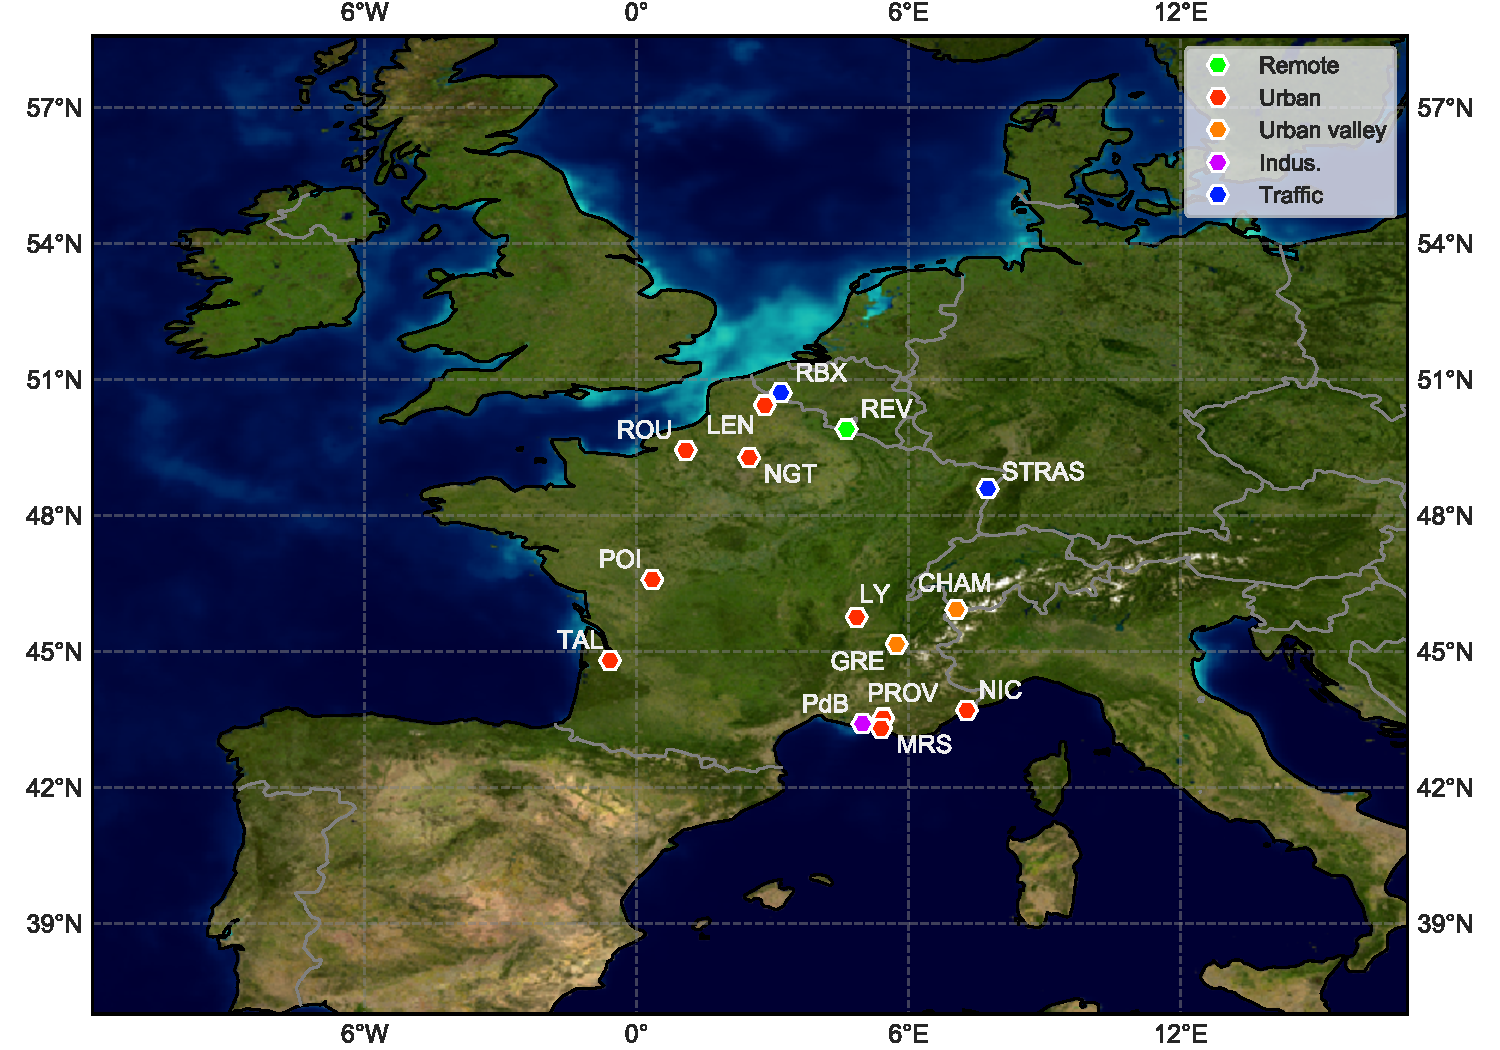
\includegraphics[width=0.9\linewidth]{chapter03/fig1.pdf}
    \caption{
        Map showing he geographical location of the 15 selected sites. Color
        codes denote the typology of the site:  green, remote; red, urban;
        orange, urban valley; magenta, industrial; blue, traffic.
    }
    \label{fig:fig1}
\end{figure}

\begin{sidewaystable}
    \centering
    \caption{Characteristics of the 15 PM sampling sites investigated in the present~study.}
    \label{tab:tab1}
    % \tablesize{\footnotesize}
    \begin{tabular}{lcp{0.11\textwidth}cccp{0.15\textwidth}}
        \toprule
        \textbf{Sampling Site}    & \textbf{Code} & \textbf{Coordinates} & E\textbf{levation}                                  & \textbf{Period }                           & \textbf{N samples} & \textbf{Typology}\\
        \midrule
        Revin            & REV  & \ang{49;55;00.00}N\newline\ang{4;38;29.00}E & \SI{395}{m} & 02 Jan 2013$\rightarrow$01 Jun 2014 & 168       & remote\\%NOTE: Please confirm all dates are in the format DD Month YYYY
        Bordeaux-Talence & TAL  & \ang{44;48; 2.01}N\newline\ang{0;35;17.01}W & \SI{ 20}{m} & 02 Feb 2012$\rightarrow$07 Apr 2013 & 154       & urban background\\
        Lyon             & LY   & \ang{45;45;27.82}N\newline\ang{4;51;15.15}E & \SI{160}{m} & 03 Jan 2012$\rightarrow$31 Dec 2012 & 115       & urban background\\
        Poitiers         & POI  & \ang{46;34;48.80}N\newline\ang{0;20;25.34}E & \SI{106}{m} & 16 Nov 2014$\rightarrow$29 Dec 2015 & 110       & urban background\\
        Nice             & NIC  & \ang{43;42; 7.48}N\newline\ang{7;17;10.53}E & \SI{  1}{m} & 04 Jun 2014$\rightarrow$29 Jun 2016 & 184       & urban background\\
        Marseille        & MRS  & \ang{43;18;18.84}N\newline\ang{5;23;40.89}E & \SI{ 64}{m} & 11 Jan 2015$\rightarrow$27 Jun 2016 & 102       & urban background\\
        Aix-en-Provence  & PROV & \ang{43;31;49.04}N\newline\ang{5;26;29.00}E & \SI{180}{m} & 18 Jul 2013$\rightarrow$13 Jul 2014 & 56        & urban background\\
        Nogent sur Oise  & NGT  & \ang{49;16;35.00}N\newline\ang{2;28;56.00}E & \SI{ 28}{m} & 02 Jan 2013$\rightarrow$02 Jun 2014 & 155       & urban background\\
        Rouen            & ROU  & \ang{49;25;41.40}N\newline\ang{1;03;29.10}E & \SI{  6}{m} & 02 Jan 2013$\rightarrow$01 Jun 2014 & 162       & urban background\\
        Lens             & LEN  & \ang{50;26;12.60}N\newline\ang{2;49;36.70}E & \SI{ 47}{m} & 02 Jan 2013$\rightarrow$01 Jun 2014 & 167       & urban background\\
        Grenoble         & GRE  & \ang{45;09;42.84}N\newline\ang{5;44;08.15}E & \SI{214}{m} & 02 Jan 2013$\rightarrow$29 Dec 2014 & 240       & urban background\newline\& alpine valley\\
        Chamonix         & CHAM & \ang{45;55;21.00}N\newline\ang{6;52;12.00}E & \SI{1038}{m}& 02 Nov 2013$\rightarrow$31 Oct 2014 & 115       & urban background\newline\& alpine valley\\
        Port de Bouc     & PdB  & \ang{43;24;07.99}N\newline\ang{4;58;55.99}E & \SI{  1}{m} & 01 Jun 2014$\rightarrow$27 Jun 2016 & 185       & urban background\newline\& industrial\\
        Roubaix          & RBX  & \ang{50;42;23.60}N\newline\ang{3;10;50.50}E & \SI{ 10}{m} & 20 Feb 2013$\rightarrow$26 May 2014 & 157       & urban traffic\\
        Strasbourg       & STG  & \ang{48;34;24.25}N\newline\ang{7;45;07.60}E & \SI{139}{m} & 02 Apr 2013$\rightarrow$08 Apr 2014 & 78        & urban traffic\\
        \bottomrule
    \end{tabular}
\end{sidewaystable}


\subsection{PMF~Methodology}%
\label{sub:pmf_methodology}

\subsubsection{PMF~Model}%
\label{ssub:pmf_model}

The U.S. Environmental Protection Agency (US-EPA) PMF5.0 software~\autocite{norrisEPA2014}
was used in the present study to achieve the PM source apportionment. Similar to other RM
approaches, PMF aims at solving the mass conservation between the measured species
concentrations and source emissions as a linear combination of factors $p$, species
profile $f$ of each source,  and the~amount of mass $g$ contributed to each individual
sample, following Equation~(\ref{eq:PMF}):

\begin{equation}
    \label{eq:PMF}
    X_{ij} = \left( \sum_p g_{ip} \times f_{pj} \right) + e_{ij}
\end{equation}

where $X_{ij}$ represents the measured data for species $j$ in sample $i$, and~$e_{ij}$ is
the residual of each sample and species not fitted by the model.  Detailed information on
the PMF methodology can be found elsewhere
~\autocite{paateroPositive1994,paateroLeast1997}. Briefly, a~multivariate factor analysis
was applied to decompose the matrix of the chemical dataset into two matrices: factor
contributions ($G$) and factor profiles ($F$), each factor to be ascribed to a specific
aerosol fraction (i.e., factor), that may be attributed to a source.  It is based on a
weighted least square fit, where the weights are derived from the analytical uncertainty,
and~provides the optimal solution by minimizing the function $Q$, given by
Equation~(\ref{eq:PMFQ}):

\begin{equation}
    \label{eq:PMFQ}
    Q = \sum_i \sum_j \left(\frac{e_{ij}}{\sigma_{ij}}\right)^2
\end{equation}

where $\sigma_{ij}$ represents the measurement uncertainty of each data~point.

\subsubsection{Input Variable and~Uncertainties}%
\label{ssub:input_variable_and_uncertainties}

Selection of the input variables was done based on the percentage of values above
detection limit (DL) (using \SI{60}{\percent} as a minimum threshold), and~the value of
the signal-to-noise ratio (S/N) for each species~\autocite{paateroDiscarding2003}.
Table~\ref{tab:input_var} presents the PMF input variables selected for this work. This
dataset notably includes EC, major ions, molecular organic markers (MSA, levoglucosan, and
mannosan), and~a selection of metals or trace elements. Assuming that they mainly
originate from the same sources---i.e.,~primary biogenic emissions--- sorbitol, arabitol
and mannitol concentrations were summed and labeled as
polyols~\autocite{samakePolyols2019}. Furthermore, \emph{OC*} was determined by
subtracting the carbon concentrations of the specific organic markers to total \emph{OC}
concentrations, so that they are not accounted twice:

\begin{equation}
    OC^* = OC - ([MSA]\times0.12+[polyols]\times0.40+[levoglucosan]\times0.44+[manosan]\times0.44),
\end{equation}

where the coefficient are the carbon mass par unit of~mass.

The different variables were categorized in the model based on their mean signal-to-noise
ratio (S/N) as follows: ``strong'' if $S/N>2$, ``weak'' if $0.2\leq S/N\leq2$, and~``bad''
if $S/N<0.2$. For~a given site, variables classified as ``weak'' were downweighted
following PMF5.0 algorithms, while variables classified as ``bad'' were excluded from the
PMF analysis. The~\PM{} variable was classified as a total variable (with corresponding
uncertainties increased by a factor of 3)   to evaluate the contribution of the identified
factors to \PM{} data.  Extensive preliminary work was conducted to harmonize the
estimation of uncertainties of the different input variables $\sigma_{ij}$, based on the
uncertainty calculation equation proposed by~\textcite{gianiniComparative2012},
as~described by Equation~(\ref{eq:gianini}):

\begin{equation}
    \label{eq:gianini}
    \sigma_{ij} = \sqrt{ DL_j^2 + (CV_j\times x_{ij})^2 + (a\times x_{ij})^2 }
\end{equation}

with \emph{DL} the detection limit (twice the standard deviation of field blanks,
with~field blanks samples representing about \SIrange{5}{10}{\percent} of the actual
number samples); $x_{ij}$ the concentration of species $j$ on day $i$; \emph{CV} the
coefficient of variation of species $j$; and $a$ the additional coefficient of variation.

Many trial-and-error tests were conducted with the aim of defining domains of variation of
the coefficient $a$ that are dependent on the type of analysis performed, i.e.,~to assign
a $a$ value to each category or family of chemical species analyzed. The~PMF solutions
obtained for different values of $a$ were examined   to optimize the stability of the
results as well as the geochemical reality of the solved factors. The~values eventually
retained vary between 3\% and 15\% depending on the different categories of chemical
species, as presented in Table~\ref{tab:input_var}.

It should also be noted that an uncertainty of $5/6 \times DL$ was applied for values
lower than the DL and uncertainties equal to  four times the specie concentration
geometric mean were attributed to missing or replaced values,
following~\textcite{polissarAtmospheric1998}.

\begin{table}[h!]
    \centering
    \caption{Input variables and uncertainties used in the PMF~analyses.}
    \label{tab:input_var}
    \footnotesize
    \begin{tabular}{lp{0.15\textwidth}p{0.18\textwidth}p{0.13\textwidth}p{0.25\textwidth}}
        \toprule
                        & \textbf{Carbonaceous Species} & \textbf{Water-Soluble Ions and MSA }                      & \textbf{Organic Markers}                 & \textbf{Metals and Trace Elements}\\
        \midrule
        Species         & OC*, EC              & MSA, \ce{Cl-}, \ce{NO3^-}, \ce{SO4^2-}, \ce{NH4+}, \ce{K+}, \ce{Mg^2+}, \ce{Ca^2+} & Polyols, \newline levoglucosan, \newline mannosan & Al, As, Ba, Cd, Co, Cr, Cs, Cu, Fe, La, Mn, Mo, Ni, Pb, Rb, Sb, Se, Sn, Sr, Ti, V, Zn\\
        $a$ coefficient & 0.03                 & 0.05                                             & 0.10                            & 0.15\\
        \bottomrule
    \end{tabular}
\end{table}


\subsubsection{Set of~Constraints}%
\label{ssub:set_of_constraints}

One of the limitations of PMF is related to a possible collinearity of factors due to
co-emission or co-accumulation phenomena, leading to rotational ambiguities.      To solve
this problem, specific chemical constraints based on expert geochemical knowledge can be
applied to the chemical profiles (or contributions) of PMF factors (both ``soft'' and
``hard'' pulling, as~defined in Section~\ref{sub:uncertainties_of_pmf_factors}), after~the
selection of the initial base runs. As~part of this study, a~minimal and homogeneous set
of chemical constraints  was defined, as~summarized in Table~\ref{tab:constraints}. They
were applied to the PMF analysis of each~site.

\begin{table}[h!]
    \centering
    \caption{Summary of the specific constraints applied on source-specific
    tracers in some of the identified PMF factor profiles.  SOA, secondary
organic aerosol; HFO, heavy fuel oil}
    \label{tab:constraints}
    \begin{tabular}{llcc}
        \toprule
        \textbf{Factor Profile}   & \textbf{Species }       & \textbf{Constraint}          & \textbf{Value }\\
        \midrule
        Biomass burning  & Levoglucosan   & Pull up Maximally   & \%dQ 0.50 \\
        Biomass burning  & Mannosan       & Pull up Maximally   & \%dQ 0.50 \\
        Primary traffic  & Levoglucosan   & Set to 0            & 0 \\
        Primary traffic  & Mannosan       & Set to 0            & 0 \\
        Primary biogenic & Levoglucosan   & Set to 0            & 0 \\
        Primary biogenic & Mannosan       & Set to 0            & 0 \\
        Primary biogenic & Polyols        & Pull up Maximally   & \%dQ 0.50 \\
        Primary biogenic & EC             & Pull down Maximally & \%dQ 0.50 \\
        Marine SOA       & Levoglucosan   & Set to 0            & 0 \\
        Marine SOA       & Mannosan       & Set to 0            & 0 \\
        Marine SOA       & Polyols        & Pull down Maximally & \%dQ 0.50 \\
        Marine SOA       & MSA            & Pull up Maximally   & \%dQ 0.50 \\
        Marine SOA       & EC             & Pull down Maximally & \%dQ 0.50 \\
        HFO combustion   & Levoglucosan   & Set to 0            & 0 \\
        HFO combustion   & Mannosan       & Set to 0            & 0 \\
        HFO combustion   & Polyols        & Set to 0            & 0 \\
        HFO combustion   & MSA            & Set to 0            & 0 \\
        Sea-salt         & Ratio \ce{Mg^2+/Na+} & Sea-salt ratio 0.119& \%dQ 0.50\\
        \bottomrule
    \end{tabular}
\end{table}

\subsection{Criteria for Valid~Solutions}%
\label{sub:criteria_for_valid_solutions}

Solutions with a total number of factors from 6 to 12 were examined   to capture the
optimal number of factors for each site. Various statistical performance parameters to
evaluate the robustness and relevance of the selected final solution were studied
according to the recommendations of the European guide on air pollution source
apportionment with receptor models~\cite{belisEuropean2014}, as~well as the geochemical
evaluation of the solution. Briefly, these parameters are summarized as~follows:

\begin{itemize}
    \item Evolution of the ratio Qtrue/Qrobust (<1.5). The~solutions retained
        on all 15 sites have a Qtrue/Qrobust ratio of 1, indicating a zero
        impact of outliers on the results.
    \item The weighted residuals for most of the species have a normal centered
        distribution and between $\pm4$, indicating an overall good modeling of
        most variables.
    \item Evaluation of the statistical representativity of the solution and
        sensitivity to noise and single point in the data from the bootstrap
        test (BS) for 100 successive iterations of the model and for a minimum
        correlation $r^2$ of 0.6.
    \item Evaluation of the rotational ambiguity and sensitivity of the
        solution to small changes from (default dQ of the software) the
        Displacement Test (DISP) proposed by the software.
    \item Evaluation of the geochemical meaning and the physical reality of
        extracted factor profiles based on the knowledge of the chemical
        footprints of the sources, their specific tracers, the~temporal
        variability (daily, weekly and seasonally), and~the characteristics of the
        site studied.
    \item Statistical evaluation and precision for constrained solutions
        regarding the BS and \%dQrobust as well as DISP.
\end{itemize}

Further discussions on the BS and DISP approaches are proposed in
Section~\ref{sub:uncertainties_of_pmf_factors}. 

\subsection{Test of Similarity between Chemical~Profiles}%
\label{sub:test_of_similarity_between_chemical_profiles}

Since factors in the different PMF were labeled with the same name due to their chemical
composition and time variation, a~tool was needed to objectively assess the homogeneity of
their chemical profiles. The~similarities between the factors or sources were tested with
both the Pearson distance (PD) and the Similarity Identity Distance (SID),
following~\textcite{belisNew2015} and using Python 3.5. The~PD is equal to $1-r^2$ where
$r^2$ is the Pearson coefficient and SID is defined by Equation~(\ref{eq:SID}):

\begin{equation}
    \label{eq:SID}
    SID = \frac{\sqrt{2}}{m} \sum_{j=1}^m \frac{|x_j - y_j|}{x_j+y_j},
\end{equation}

with $x$ and $y$ the relative mass to the PM of  two different factors or sources and $m$
the number of common specie in $x$ and $y$.

Shortly, these two metrics aim to compare  two  profiles based on their common chemical
relative mass composition. The~PD is highly sensitive to variation in the major mass
fractions of the PM, while the SID is equally sensitive to all components. $PD < 0.4$ and
$SID < 1$ are considered as acceptable criteria for profile similarity, according
to~\textcite{pernigottiDeltaSA2018}.

\section{Results and~Discussions}%
\label{sec:results_and_discussions}

The outputs of the SOURCES project consist of a large database, which cannot be
exhaustively discussed in a single paper. Here, we present an overview of obtained PMF's
results, give some examples of factor's behaviors, and focus on the statistical evaluation
of the solutions as well as on the comparability of various factors. However, all the
results---including time-series and factors profiles along with their corresponding
uncertainties--- have been made interactively available online at
\url{http://pmsources.u-ga.fr}. This application is proposed as Supplementary Material for
the present~paper.  

It should be noted that the harmonized methodology used for the purpose of this study may
lead to slight discrepancies when compared to results obtained in the case of PMF analysis
performed specifically at a given site, as~discussed for instance
in~\textcite{favezTraitement2017}.

\subsection{Identification  of~Factors}%
\label{sub:identification_of_factors}

The number of selected factors varied between 8 and 11 depending on the site.  Among these
factors, nine  were identified at most of the locations: biomass burning, exhaust and
non-exhaust road transport emissions (primary traffic), secondary aerosols dominated by
ammonium nitrate and ammonium sulfate (nitrate-rich and sulfate-rich, respectively),
primary biogenic particles, secondary organic aerosols (SOA) from marine biogenic
emissions (marine SOA), fresh and/or aged sea-salt, and~mineral dusts. It is noteworthy
that this harmonized methodology enables   identifying such a large and common set of
factor at the national scale. Two other minor factors   were exclusively identified at a
few sites and seem to be specific of local sources: industrial emissions (at five sites)
and emission related to combustion of heavy fuel oil (HFO) (at three sites). 

All of these chemical profiles  were identified and attributed to different sources (or
source categories) mainly based on the presence of specific chemical tracers or
combination of markers, as~presented in Table~\ref{tab:species}. In~some cases, it was
impossible to separate two factors among   the ones listed in Table~\ref{tab:species},
and~they were named as a combination of both of them (Figure~\ref{fig:fig2}). The~main
chemical characteristics of the factors identified at all 15 sites, as~well as the
particularities observed on some sites, may be found in the
\href{http://pmsources.u-ga.fr}{web app}, together with their concentrations time~series.

One of the specificities of theses PMF is the use of organics species (polyols and MSA
notably). Discussion on the identification of the factors may be found in previous paper
~\autocite{srivastavaSpeciation2018,salamehSources2018,salamehImpacts2015,chevrierChauffage2016,gollyEtude2014,wakedSource2014},
where the same criteria are applied. However, we would like to mention the presence of Se
in the sulfate rich factor. Indeed, Se is not often used in PMF studies together with
organics. In~this study, \SI{23\pm15}{\percent} of the Se was associated to the sulfate
rich factor, together with \SI{13\pm6}{\percent} of the OC*. Such association of Se,
\ce{SO4^2-} and OC is already documented for soil~\autocite{toluDistribution2014} as well
for the emission of Se and S from marine algae~\autocite{luxemStudying2017}. It has also
been reported that abiotic condition could lead to the formation of volatile Se when
associated with organic acid
~\autocite{amourouxFormation2000,guoPhotochemical2003,guoUV2003}. Then, the~sulfate rich
factor may not be only an inorganic aerosol but may also be induced by the formation of
secondary organics.

\begin{table}[ht]
    \centering
    \caption{Summary of the characteristic marker species used to identify PMF~factors.}
    \label{tab:species}
    \begin{tabular}{ll}
        \toprule 
        \textbf{Identified Factors}  & \textbf{Specific Markers and Indicators}\\
        \midrule
        Biomass burning      & Levoglucosan, mannosan, \ce{K+}, OC, EC\\
        Primary traffic      & EC, OC, Ba, Cr, Co, Cu, Fe, Mo, Pb, Sb, Sn, Zn\\
        Nitrate rich         & \ce{NO3^-}, \ce{NH4+}\\
        Sulfate rich         & \ce{SO4^2-}, \ce{NH4+}, Se, OC\\
        Primary biogenic     & Polyols\\
        Marine SOA           & MSA\\
        Dust                 & \ce{Ca^2+}, Al, Ba, Co, Cu, Fe, Mn, Pb, Sr, Ti, Zn\\
        Sea-salt             & \ce{Na+}, \ce{Mg^2+}, \ce{Ca^2+}, \ce{Cl-}\\
        Aged sea-salt        & \ce{Na+}, \ce{Mg^2+}, \ce{NO3^-}, \ce{SO4^2-}\\
        Industries           & As, Cd, Cr, Cs, Co, Ni, Pb, Rb, Se, V, Zn\\
        Heavy fuel oil (HFO) & V, Ni, \ce{SO4^2-}, EC\\
        \bottomrule
    \end{tabular}
\end{table}

\subsection{Major Source Contributors To~PM}%
\label{sub:major_source_contributors_to_pm}

Figure~\ref{fig:fig2} presents the yearly mass contributions of the different factors
identified at all sites, in both   absolute (top) and relative 
(bottom) contributions. The~all-sites average ranked contributions of the main PM factors are
presented in Figure~\ref{fig:fig3}.

The average concentration of \PM{} for each site ranged from \SI{13.0}{\concum} for the
rural site of REV to \SI{23.3}{\concum} for the traffic site of RBX, with~an average
concentration of \SI{17.6\pm2.6}{\concum}.  As already pointed out in previous recent
studies conducted at French sites
\autocite{wakedSource2014,bressiSources2014,petitSubmicron2014,salamehSources2018,srivastavaSpeciation2018,weberApportionment2018},
one of the main PM factor is biomass burning, with~an average contribution of
\SI{2.9\pm1.5}{\concum} (\SI{17\pm9}{\%} of \PM{} mass), coming mainly from residential
heating. This is particularly true for Alpine valley sites, as~exemplified with the CHAM
site in this study, where it reaches \SI{45}{\percent} of the total \PM{} mass
(Figure~\ref{fig:fig2}). We also clearly observed the large contributions of \PM{} formed
through secondary processes, namely the nitrate-rich and the sulfate-rich factors,
representing on average \SI{3.0\pm1.6}{\concum} (\SI{17\pm8}{\percent}) and
\SI{2.6\pm0.7}{\concum} (\SI{15\pm4}{\percent}), respectively. Since such factors impact
all of the metropolitan France territory, it   suggests  the importance of large-scale
processes at the European scale,  especially during PM pollution events in the late
winter-early spring period
~\autocite{petitTwo2015,petitBlack2017,srivastavaSpeciation2018}).  The~primary traffic
factor represents another important fraction, with~a yearly contribution of
\SI{2.6\pm1.2}{\concum} (\SI{15\pm7}{\percent}).  It should be noted that this factor was
assessed to comprise oxidized compounds formed rapidly after emission, but~to miss some of
the secondary species (e.g., ammonium nitrate, SOA) partly originating from precursors
and/or oxidative species within exhaust smoke, such as high-volatility organic and
nitrogen gaseous compounds.  As another primary anthropogenic source, a~pure HFO factor
was observed for only  three  locations, with~the highest contribution to \PM{} (about
\SI{5}{\percent}) at the industrial site of PdB.  Finally, some industrial related PM was
found  at  five  sites, but~the exact types of industrial activity were not~identified.

Considering natural particles, the~dust factor was identified as a large contributor at
almost all sites ($n=13$), representing on average \SI{2.3\pm1.0}{\concum}
(\SI{13\pm4}{\percent}). However, this latter factor could possibly be considered as a
mixing between terrigenous aerosols and mineral particles linked to human activities
(e.g., building works, resuspension due to road transport, etc.), since it includes
variable amounts of trace elements depending on the site. The~primary biogenic and marine
SOA factors--- traced by polyols and MSA, respectively---represent \SI{1.2\pm0.5}{\concum}
(\SI{7\pm3}{\%}) and \SI{0.6\pm0.2}{\concum} (\SI{4\pm1}{\%}) on a yearly average and
display the lowest dispersion among all the sites studied, suggesting common large-scale
processes for these two factors. An~extensive discussion on the primary biogenic factor
for these sites can be found in~\textcite{samakePolyols2019}.  The~fresh sea-salt fraction
display an average concentration of \SI{1.1\pm0.4}{\concum} (\SI{6\pm2}{\%}) while the
aged sea-salt factor was observed at almost all sites, with~an average concentration of
\SI{1.5\pm0.9}{\concum} (\SI{8\pm4}{\%}) (Figure~\ref{fig:fig3}). This last result
strengthens the importance of the secondary processes that occurs during the aging of
natural aerosols, possibly leading to internal mixing with anthropogenic emissions.
Similarly, a~marine/HFO factor---notably containing sulfate, vanadium, sodium and
chloride---was observed at three coastal sites, pointing   to substantial influence of
shipping emissions at these~sites. 

\begin{figure}[ht]
    \centering
    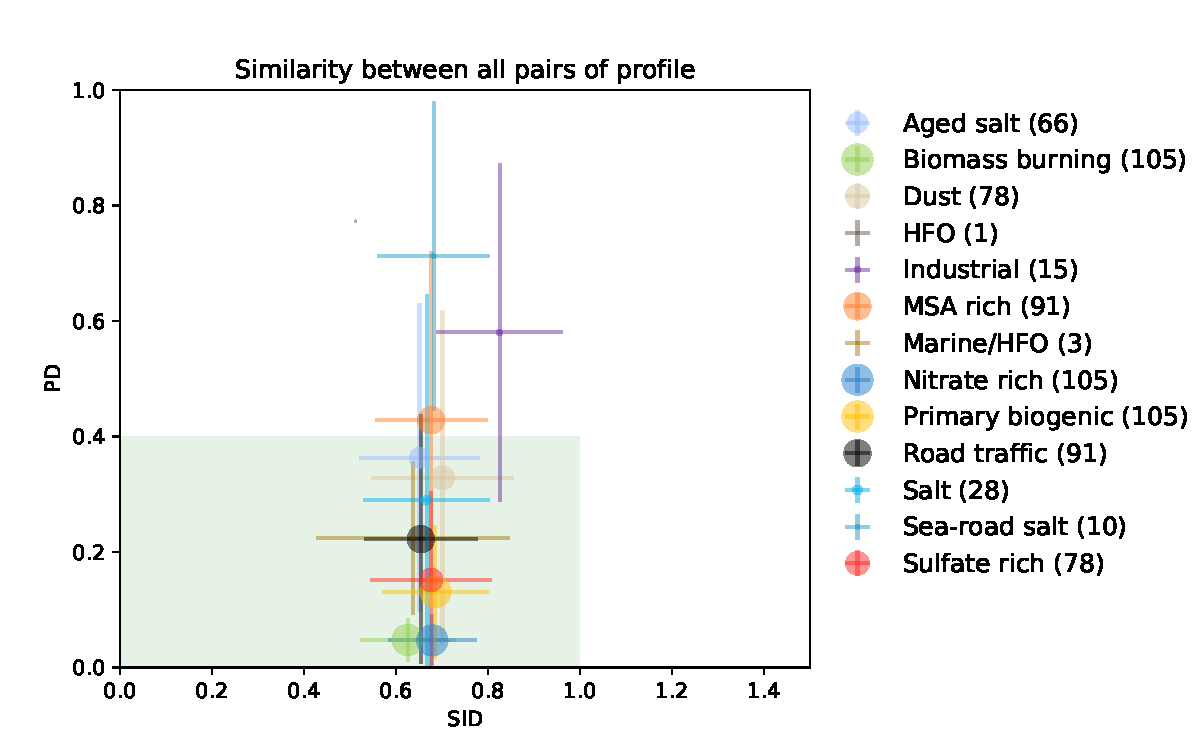
\includegraphics[width=1\linewidth]{chapter03/fig2.pdf}
    \caption{Yearly average contributions from the constrained runs in
        \si{\concum} (\textbf{top}) and \si{\percent} (\textbf{bottom}) of the identified factors to
        \PM{} mass at each of the sites studied, grouped by typology (remote, urban,
urban valley and traffic).} 
\label{fig:fig2}
\end{figure}

\begin{figure}[ht]
    \centering
    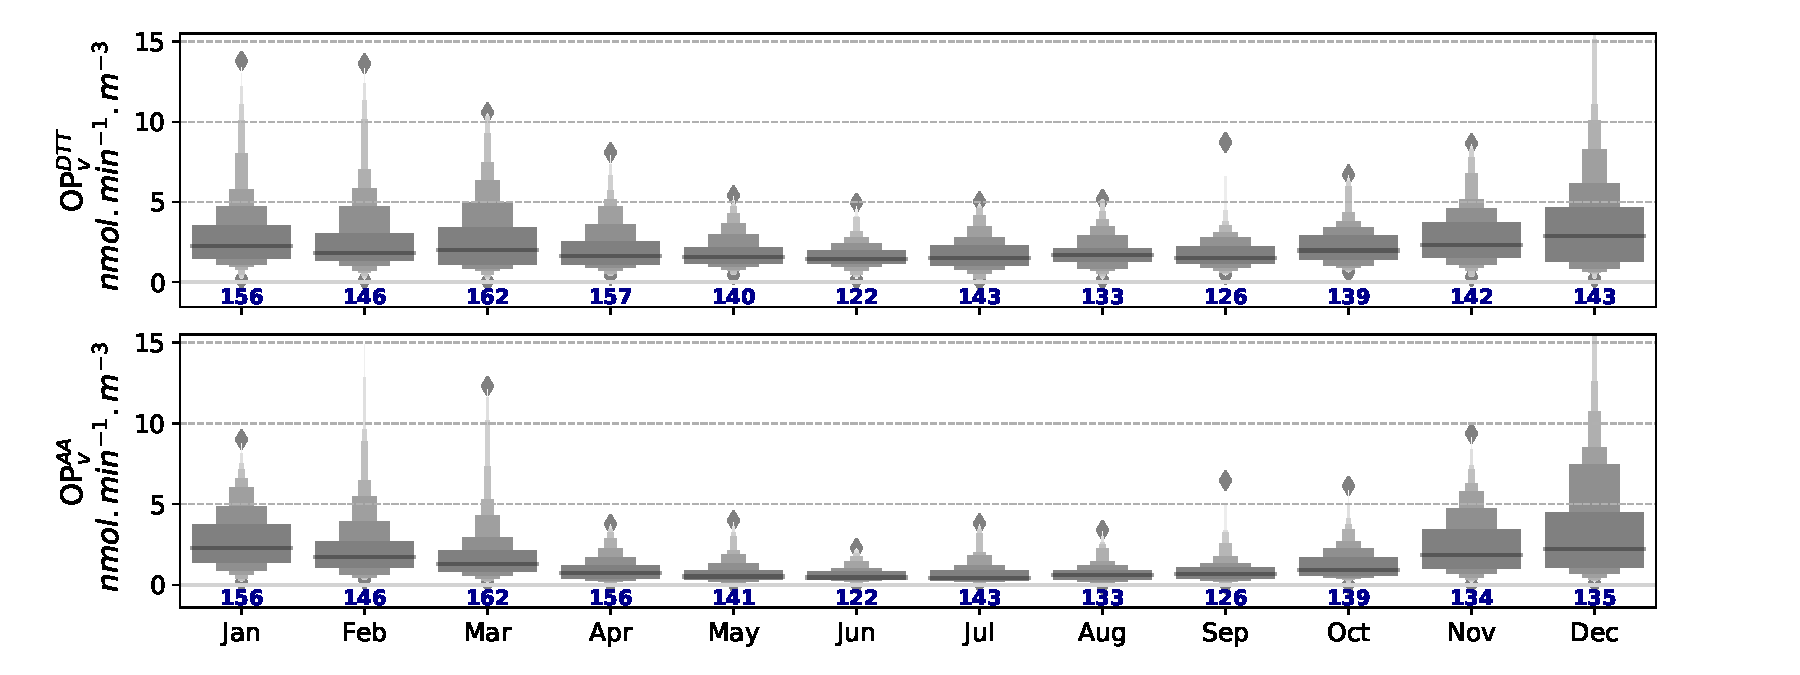
\includegraphics[width=1\linewidth]{chapter03/fig3.pdf}
    \caption{Average daily mass concentrations (\si{\concum}) of the main PMF factors
        (observed at least at 10~sites) obtained in the constrained runs in
        this study. Error bars indicate the standard deviation between sites
        and $n$ denotes the number of sites where the factors were identified.}
    \label{fig:fig3}
\end{figure}


\subsection{Seasonality of the~Contributions}%
\label{sub:seasonality_of_the_contributions}

Since it is not possible to present all the results in this paper, we encourage the reader
to refer to the online view app to browse the different time series and chemical profiles.
Among~the factors that present a strong seasonality (nitrate rich, biomass burning,
primary biogenic and marine SOA) we choose to highlight the seasonal contributions of the
biomass burning (main contribution during winter) and the primary biogenic (main
contribution during summer) (Figures~\ref{fig:fig4} and~\ref{fig:fig5}, respectively).

With about {35}{\%} of the \PM{} mass during winter and less than {2}{\%} during summer
(see Figure~\ref{fig:fig4}), the~biomass burning factor shows the strongest seasonality
among all factors identified. At~the two sites investigated in the Alpine valley, and~due
to frequent inversion layers in winter, the~contribution of the biomass burning can reach
up to {70}{\%} of the total \PM{} mass in the cold season, as~already mentioned in
previous studies in the
Alps~\autocite{favezIntercomparison2010,bonvalotEstimating2016,srivastavaSpeciation2018,herichOverview2014}.

Conversely, the~primary biogenic factor can contribute to a significant amount of \PM{}
during the warm months, with~an average contribution to \PM{} of \SI{13\pm8}{\percent}
(min \SI{1.5}{\percent}, max \SI{33}{\percent} among the sites studied) during summertime,
as~shown in Figure~\ref{fig:fig5}. A~detailed study about the seasonal and spatial
variations of the primary biogenic factor resulting from these PMF analyses can be found
in~\mbox{\textcite{samakePolyols2019}}.

\begin{figure}[ht]
    \centering
    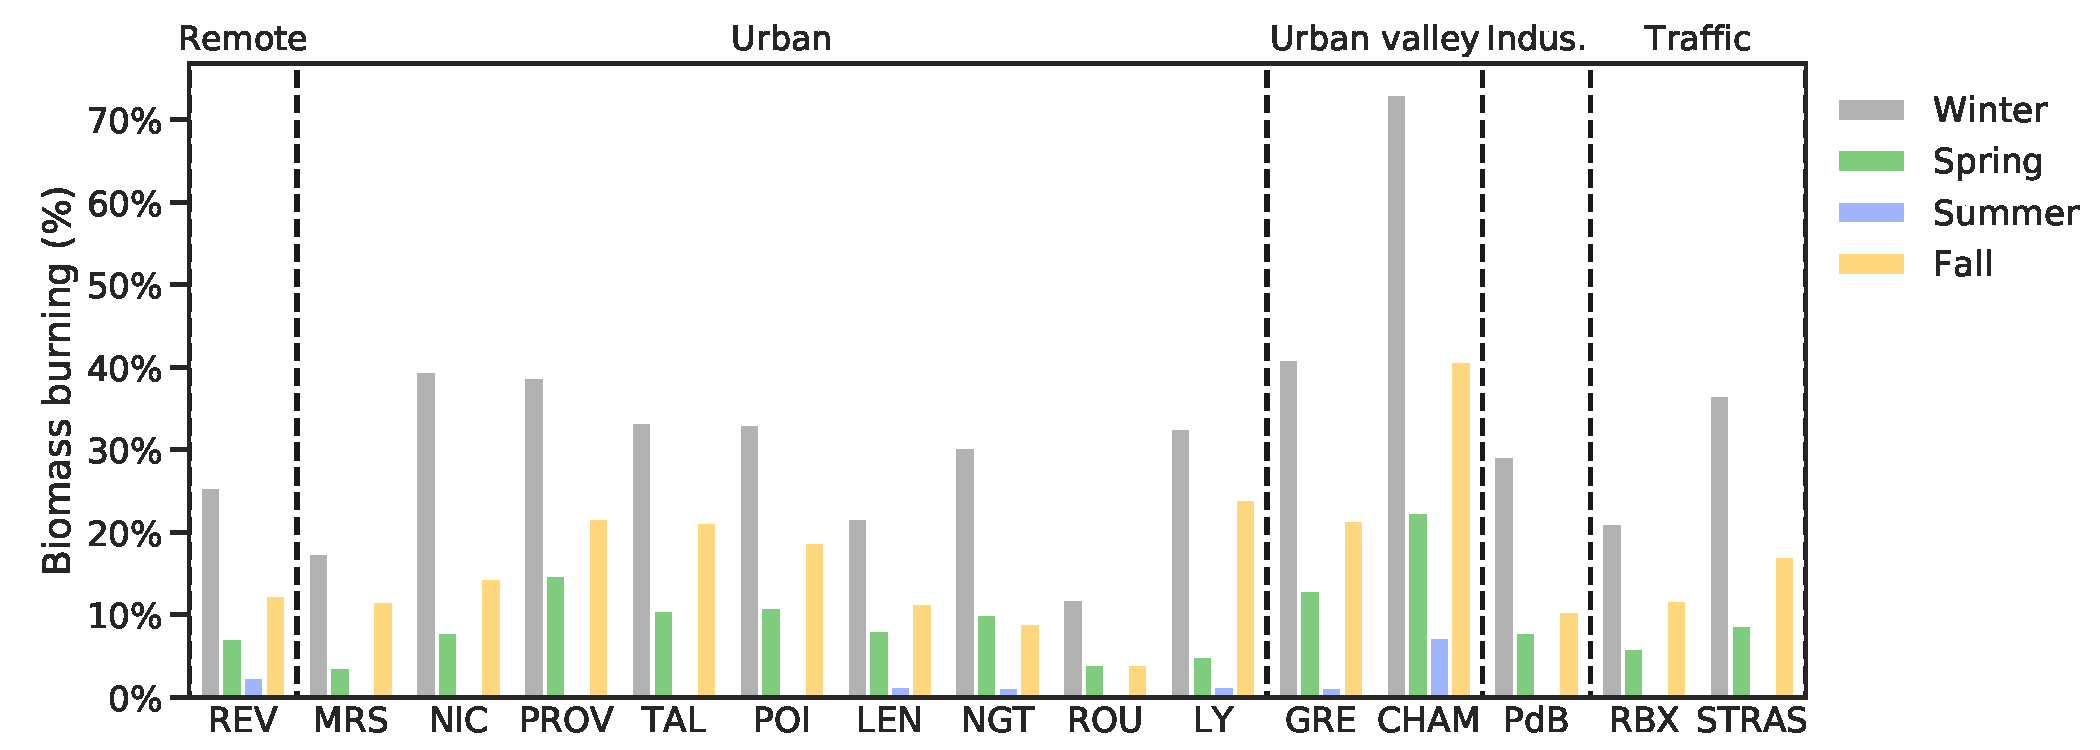
\includegraphics[width=1\linewidth]{chapter03/fig4.pdf}
    \caption{Biomass burning seasonal contributions (in \si{\percent}) to the total PM mass
    from the constrained~runs.}
    \label{fig:fig4}
\end{figure}

\begin{figure}[ht]
    \centering
    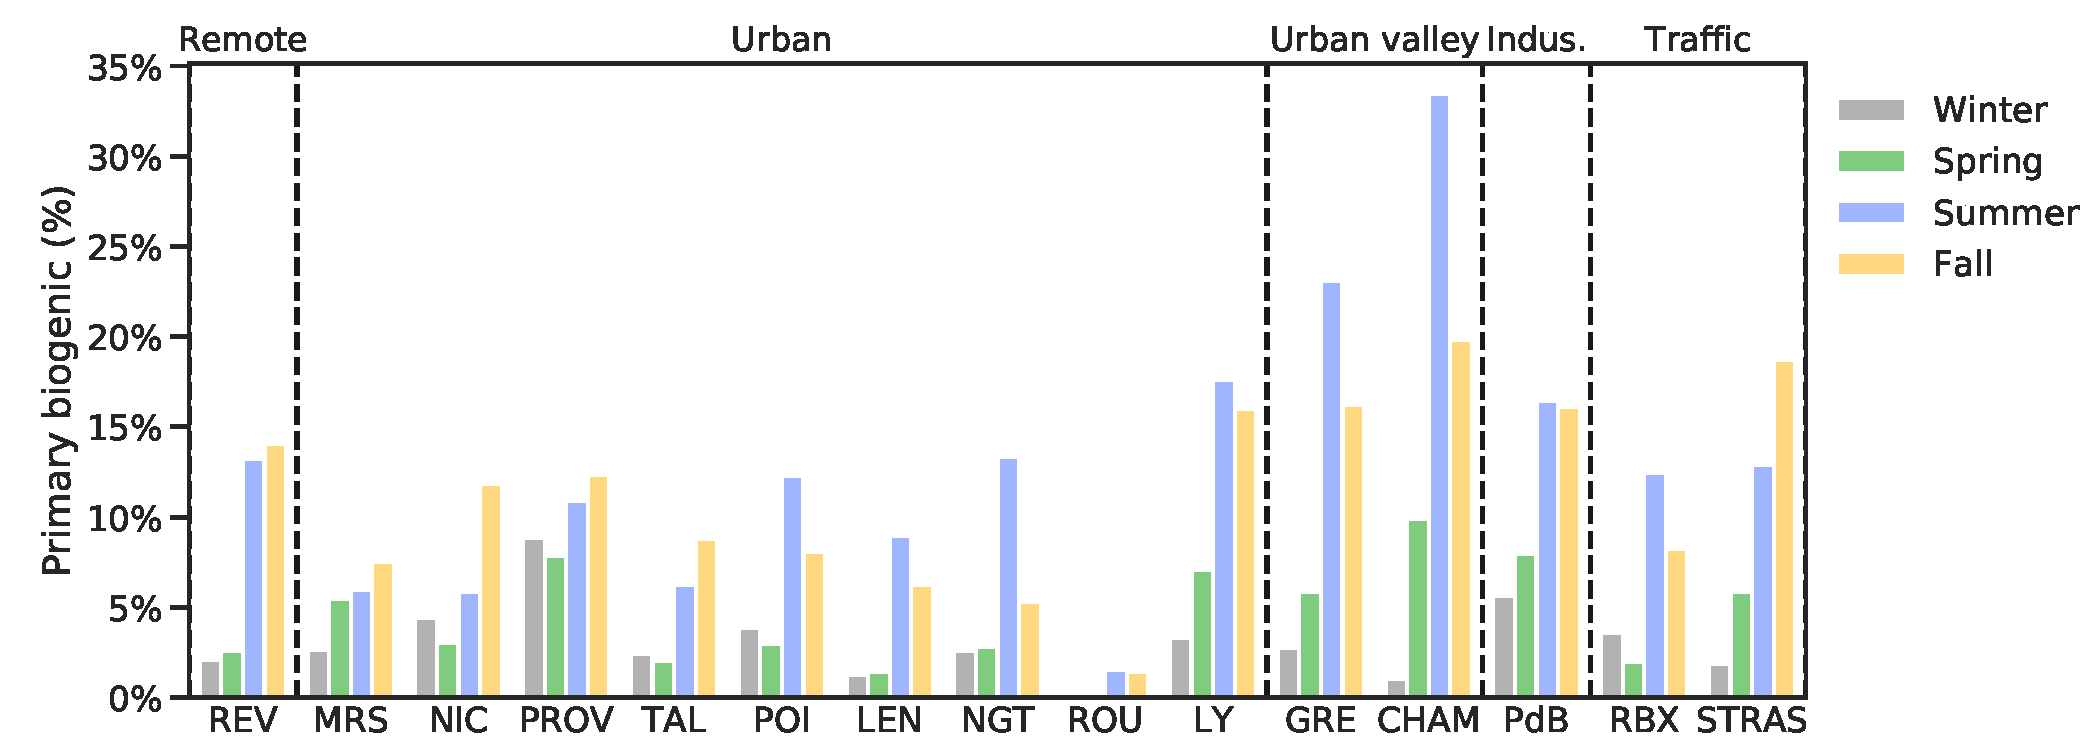
\includegraphics[width=1\linewidth]{chapter03/fig5.pdf}
    \caption{Primary biogenic seasonal contributions (in \si{\percent}) to the total PM mass
    from the constrained runs.}
    \label{fig:fig5}
\end{figure}


\subsection{Uncertainties of PMF Factors}%
\label{sub:uncertainties_of_pmf_factors}

In factor analysis, three sources of uncertainties can arise from: (1) random errors in
data values linked to measurement uncertainties: (2) rotational ambiguity due to possible
multiple acceptable solutions; and  (3) modeling errors, such as mis-specification of the
model compare to the real processes in atmosphere~\autocite{belisEuropean2014}.

To quantify the uncertainties of the results at one site (internal uncertainties), and~the
variability of the factor profiles, we performed both bootstrap (BS) and displacement
(DISP) analyses. Shortly, BS randomly resample the $X$ matrix and perform a new PMF run,
then try to map each new BS-factor to the reference run, according to the correlation
between the contributions of factors. A~threshold correlation coefficient of 0.6 was used
for all sites in this study. BS gives an estimation of uncertainties linked to sampling
artifact and measurement uncertainties. DISP analysis estimates the rotational ambiguity
by lowering and majoring each species in every factor up to a given variation of the $Q$
value dQmax. The~reader may refer to~\textcite{paateroMethods2014} for more details about
DISP computation in EPA PMF5.0. Here, BS and DISP analyses were applied in both base runs
and constrained runs, i.e.,~before and after applying the constraints listed in
Table~\ref{tab:constraints}.


\subsubsection{Statistical Stability of the~Solutions}%
\label{ssub:statistical_stability_of_the_solutions}

In this study, all base cases solutions (i.e., without constraints) reached high BS
values, the~lowest one being {77}{\%} (Table~\ref{tab:BSmapping}).  Hence, the~PMF base
solution for all sites already presents very good BS mapping results that largely agree
with the general recommendations of the European guide on air pollution source
apportionment with receptor models~\autocite{belisEuropean2014}. Moreover, we
systematically observed improvement in BS mapping when applying constraints
(Table~\ref{tab:BSmapping}).  Considering all the sites, the~minimum value of BS for
constraint solutions was \SI{83}{\percent}. It means that, even if the base cases were
good enough to differentiate specific factors, the~expert knowledge added through the use
of specific constraints helped the model to ``clean'' the factors and improve the
stability of the solutions. Finally, we note that virtually no ``unmapped'' factor was
obtained during this BS sensitivity analysis (always less than {1}{\%}).  Concerning the
DISP analyses, no swap between factors was observed,   for both the base and
constrained~runs.

\begin{table}[ht]
    \centering
    \caption{
        Summary of bootstrap mapping of the base runs and of the constrained
        runs expressed as percent of correct mapping bootstrap for the main
        factors identified in this study. Ranges are min and max. The~number in
        parenthesis is the number of sites where the given profile could be
        identified.
    }
    \label{tab:BSmapping}
	\footnotesize
    \begin{tabular}{lScSScS}
        \toprule
                        & \multicolumn{3}{c}{\textbf{Base Cases}} & \multicolumn{3}{c}{\textbf{Constrained Cases}}\\
\textbf{Profiles}                & {\textbf{Mean $\pm$ Std}} & \textbf{Range} & {\textbf{Unmapped}} & {\textbf{Mean $\pm$ Std}} & \textbf{Range} & {\textbf{Unmapped}}\\
        \midrule
Biomass burning (15)    & 100.0\pm0.0    & 100--100 & 0.0        & 100.0\pm0.0    & 100--100 & 0.0\\
Nitrate rich (15)       & 98.7\pm2.8     & 89--100  & 0.2        & 99.9\pm0.3     & 99--100  & 0.0\\
Primary biogenic (15)   & 99.3\pm1.3     & 96--100  & 0.0        & 99.8\pm0.8     & 97--100  & 0.0\\
Marine SOA (14)         & 95.9\pm4.9     & 83--100  & 0.7        & 100.0\pm0.0    & 100--100 & 0.0\\
Primary traffic (14)    & 97.1\pm4.8     & 85--100  & 0.0        & 98.7\pm2.8     & 89--100  & 0.0\\
Aged sea-salt (13)      & 95.8\pm4.8     & 83--100  & 0.1        & 98.5\pm2.7     & 91--100  & 0.1\\
Sulfate rich (13)       & 93.4\pm6.9     & 83--100  & 0.5        & 98.9\pm1.8     & 95--100  & 0.1\\
Dust (12)               & 94.1\pm7.3     & 77--100  & 0.7        & 97.8\pm4.8     & 83--100  & 0.1\\
Sea-salt (11)           & 99.5\pm1.5     & 95--100  & 0.0        & 99.8\pm0.6     & 98--100  & 0.0\\
Industries (5)          & 92.8\pm8.5     & 80--100  & 1.0        & 98.4\pm2.2     & 96--100  & 0.0\\
        \bottomrule
    \end{tabular}
\end{table}

\subsubsection{Uncertainties of the Profile~Composition}%
\label{ssub:uncertainties_of_the_profile_composition}

\paragraph{Impacts of the Constraints on the Uncertainties}%
\label{par:impacts_of_the_constraints_on_the_uncertainties}

The application of specific chemical constraints (see Table~\ref{tab:BSmapping}) also
improved the resolving power of the PMF and the quality of the solutions, displaying
narrower uncertainties for the contributions of chemical species in many factors.
For~instance, the~OC* concentration in the primary traffic profile of ROU   varied between
0.79 and \SI{1.65}{\concum} for the base run but only between 1.23 and \SI{1.84}{\concum}
in the constrained run, according to the BS analysis (5{th}--95{th})
(Table~\ref{tab:uncertainties_constraints}). Similar trends were observed for the
uncertainties proposed by the DISP approach and were apparent for most of the chemical
species that are proxies of a given source (Table~\ref{tab:uncertainties_constraints}
proposes some examples).

Interestingly, the~uncertainties estimated with the DISP method were almost always
narrower than the uncertainties given by the BS method. This may be explained by using
constraints that already narrowed the rotational ambiguity (lowering DISP uncertainties
range) or by the sensitivity of our datasets to specific days (increasing BS uncertainties
range).

\paragraph{Composition Uncertainties in the Chemical Profiles}%
\label{par:composition_uncertainties_in_the_chemical_profiles}

The dispersion of the concentrations of key species in different profiles was investigated
and is briefly presented here. The~external variability (from site to site) is presented
in its own section below
(Section~\ref{sub:variability_of_the_chemical_profiles_at_the_regional_scale}).  Here, we
only assessed the internal variability, i.e.,~the variability of a specie at a given site
for a given factor, and~the coefficients of variation (CV, standard deviation over the
mean) of species from the BS runs are presented in Figure~\ref{fig:fig6}, averaged from
all sites.      To minimize the impact of potential outliers in the BS runs, only the BS
values above the 5{th} percentile and below the 95{th} percentile were~used.

\begin{sidewaystable}
    \centering
    \caption{Summary of the uncertainties (in \si{\concum}) obtained from the BS
        (5{th} and 95{th} percentiles) and DISP
        (min-max) runs for a subset of species in two different factor profiles,
        the road traffic at ROU site and the biomass burning at GRE site, for both
      the base and constrained runs}
    \label{tab:uncertainties_constraints}
    \begin{tabular}{lcccccccc}
        \toprule
        & \multicolumn{8}{c}{\textbf{ROU---Primary Traffic}}\\
       \textbf{ Run} & \multicolumn{4}{c}{\textbf{Base}} & \multicolumn{4}{c}{\textbf{Constrained}} \\
        \midrule
\textbf{Species} & OC* & EC & Cu & Fe & OC* & EC & Cu & Fe\\
Reference  & 1.605 & 0.541 & 0.0104 & 0.1986 & 1.649 & 0.592 & 0.0114 & 0.221\\
BS (5{th}--95{th}) & 0.792--1.654 & 0.334--0.541 & 0.007--0.011 & 0.108--0.232 & 1.232--1.845 & 0.493--0.641 & 0.009--0.013 & 0.159--0.264\\
DISP (min-max) & 1.426--1.912 & 0.480--0.644 & 0.009--0.012 & 0.178--0.229 & 1.576--1.837 & 0.572--0.666 & 0.011--0.012 & 0.210--0.236 \\
        \toprule
        & \multicolumn{8}{c}{\textbf{GRE---Biomass Burning}}\\
\textbf{Run} & \multicolumn{4}{c}{\textbf{Base}} & \multicolumn{4}{c}{\textbf{Constrained}} \\
        \midrule
Species & OC* & EC & Levoglucosan & K+ & OC* & EC & Levoglucosan & K+\\
Reference & 1.266 & 0.434 & 0.306 & 0.057 & 1.520 & 0.563 & 0.388 & 0.059\\
BS (5{th}--95{th}) & 1.061--1.505 & 0.372--0.614 & 0.269--0.362 & 0.039--0.067 & 1.347--1.640 & 0.492--0.672 & 0.412--0.434 & 0.039--0.070\\
DISP (min-max) & 1.100--1.363 & 0.378--0.480 & 0.275--0.319 & 0.050--0.061 & 1.456--1.589 & 0.539--0.604 & 0.408--0.439 & 0.058--0.059\\
\bottomrule
    \end{tabular}
\end{sidewaystable}



For most of the main proxies of sources (i.e., specific tracers), we observed a narrow
range of possible values given by the BS and DISP, associated with low CV for the specific
tracers. This is the case for instance for the levoglucosan in the biomass burning factor
(\SI{1.6\pm0.5}{\percent}), the~MSA in the marine SOA (\SI{1.2\pm0.8}{\percent}),
the~polyols in the primary biogenic (\SI{0.1\pm0.1}{\percent}), the~Ti in the dust
(\SI{12.2\pm9.6}{\percent}), the~\ce{Na+} in the sea-salt (\SI{10.3\pm7.2}{\percent}),
NO3- in the nitrate rich (\SI{6.5\pm2.5}{\percent}) or even Cu and Sb in the primary
traffic (\SI{14.0\pm11.0}{\percent} and \SI{16.0\pm12.4}{\percent}, respectively, which
are the lowest CVs for these two metals for all factors).

However, for~non-tracers species, the~dispersion according to the BS and DISP runs could
be larger. For~instance, according to BS, the~OC* and \ce{Ca^2+} in the nitrate rich have
a CV of \SI{60.4\pm35.9}{\percent} and \SI{59.6\pm39.1}{\percent}, respectively, or~the
metals in the primary biogenic factor.

We also note that some species have an extremely large CV in some factors, notably the
\ce{NO3^-} in the sulfate rich factor (\SI{354.3\pm301.3}{\percent}). This likely
indicates some possible mixing with other factor or more generally the fact that the PMF
model did not find a well defined solution for this species in this factor. Conversely, we
can see in Figure~\ref{fig:fig6} that the main species with regard to the mass are stable
in the biomass burning factor. Notably,  ~\PM{}, OC* and EC had CVs of
\SI{12.2\pm6.8}{\percent}, \SI{12.8\pm8.9}{\percent} and \SI{25.6\pm22.9}{\percent},
respectively, an~indication that the components of this factor  were well described by the
PMF~run.

Therefore, despite high confidence in the markers and in the obtained mass fractions,
caution should be taken when scrutinizing the repartition of a given species between
factors and extrapolating specific ratio if the species present some large~uncertainties.

\begin{figure}[ht]
    \centering
    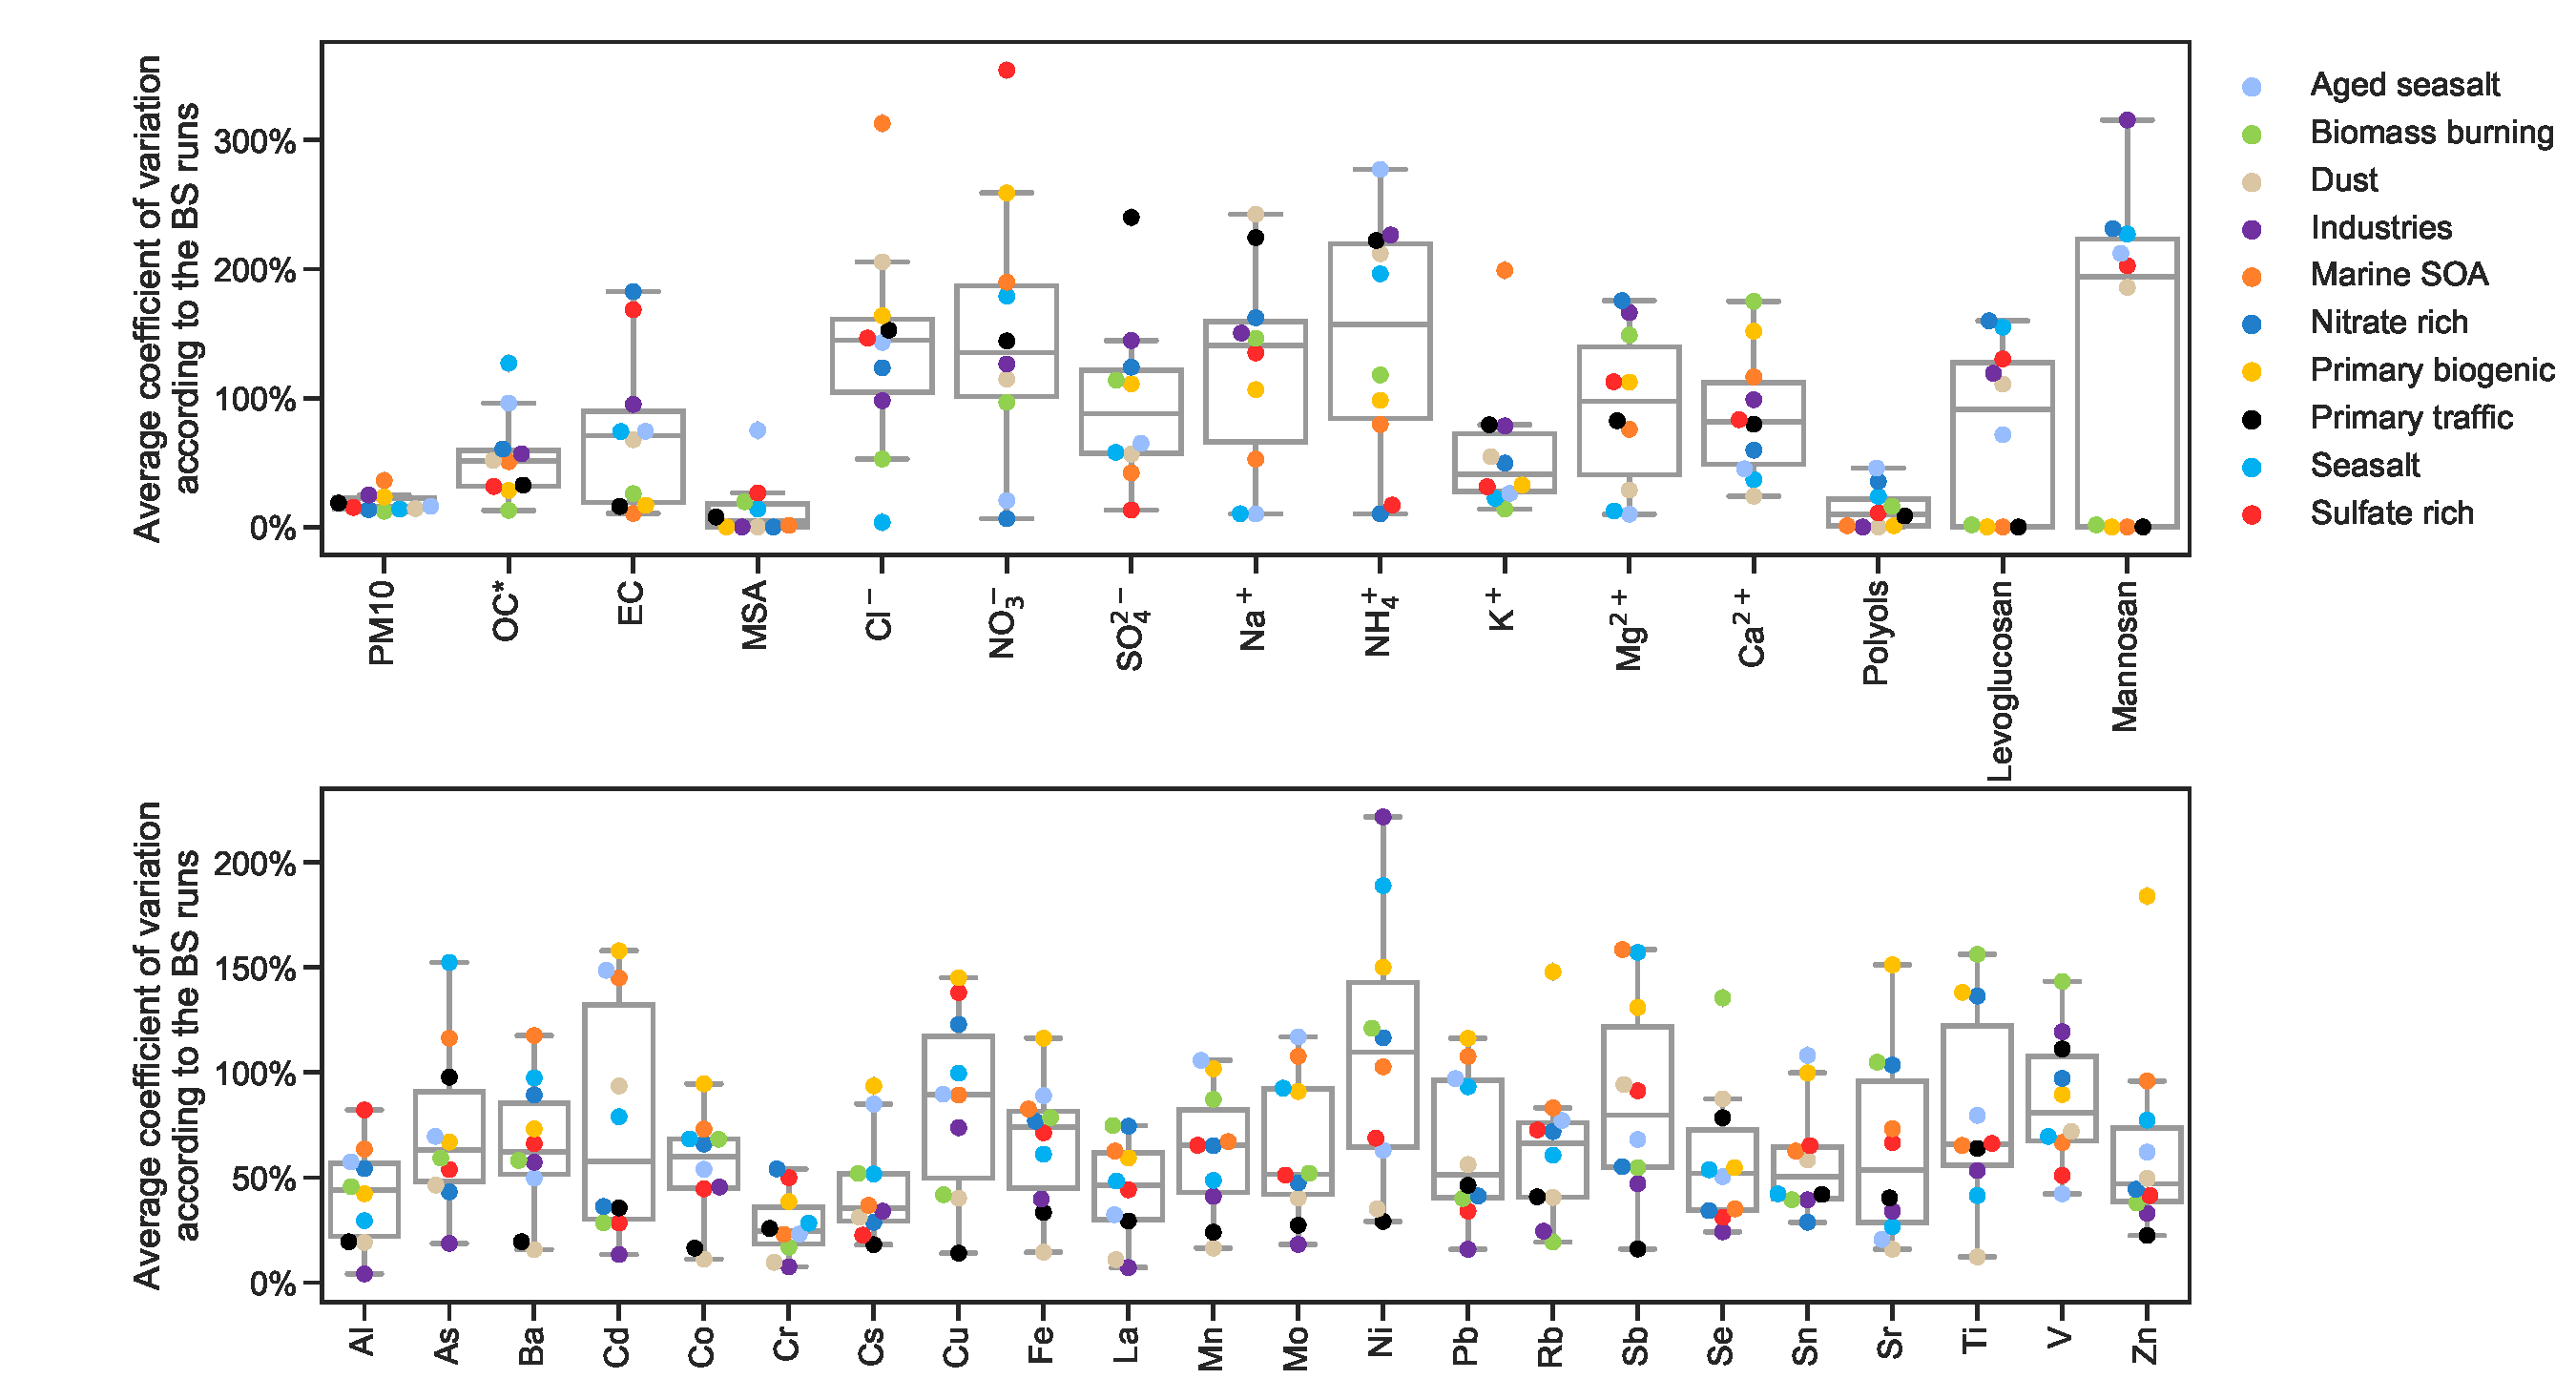
\includegraphics[width=.85\linewidth]{chapter03/fig6.pdf}
    \caption{
        Site averaged coefficient of variation of the species concentration in
        each major profile according to the BS runs. Markers are individual
        values and the box plots show  the dispersion of values.
    }
    \label{fig:fig6}
\end{figure}

\subsection{Estimation of the Uncertainties of Time Series~Concentrations}%
\label{sub:estimation_of_the_uncertainties_of_time_series_concentrations}

This section presents an attempt to express the uncertainties associated with the
concentrations of a chemical species in the time series of a specific factor contribution.
Even if during the BS runs both the $F$ and $G$ matrices  were recomputed, only the $F$
matrix was returned to the user in the EPA PMF5.0 software. The~matrix $G$ was only used
internally to map the BS factor to the base factor~\autocite{paateroMethods2014}. As~a
result, the~outcome  was an estimation of uncertainties for the $F$ matrix, but~not for
the $G$ one.  Hereafter, we propose to estimate the uncertainties for the time series of
the concentrations of a chemical species by multiplying the different concentrations given
by the uncertainties runs (BS and DISP) by the factor contribution of the reference run
$G_{ref}$:

\begin{equation}
    X'_{ERRi} = F_{ERRi} \cdot G_{ref},
\end{equation}

where $F_{ERRi}$ refers either to the $F$ matrix given by the DISP min/max run or to one
of the BS runs, $G_{ref}$ is the contribution matrix of the reference run, and~$X'_{ERRi}$
simulates the temporal concentration of species in the run $ERRi$ (DISP or BS). It should
be noted that this method only represents an approximation of the ``true'' uncertainties
of the model over the sample time series. Indeed, both the $F$ and $G$ matrix should
theoretically be modified at the same time, whereas the different $F_{ERRi}$ were
multiplied here by a constant value of $G$ for a given sample.  Therefore, samples with
high concentration ($G$) will always have higher uncertainties than sample with
low~concentration.

However, this method provides a first idea of the uncertainties in the time series and
help to visualize the uncertainties given by the BS and DISP methods.  For instance,
uncertainties (i.e., standard deviation of BS, and~DISP min/max) of the OC* in the
sulfate-rich factor obtained for the site CHAM are presented in Figure~\ref{fig:fig7},
coupling the uncertainties in the chemical profile (OC*\textsubscript{ref},
\SI{0.5423}{\concum}; OC*\textsubscript{BS}, \SI{0.568\pm0.262}{\concum}; and
OC*\textsubscript{DISP}, \SIrange{0.612}{0.934}{\concum}) and the concentrations time
series. In~this example, it may be hypothesized that the sulfate-rich factor may be mixed
with another aerosol fraction (e.g., possibly SOA) since it presents some important
uncertainties and high concentration of OC* during summertime.  Even if it may be possible
by directly tweaking the ME-2, the~solver used in EPA PMF5.0 software, it seems difficult
for the non-computers-scientist end-user to extract the different $G$ matrices. We think
that an added value to the software would be to output them during the BS process and we
encourage developers of other PMF software to ease this~process.

\begin{figure}[ht]
    \centering
    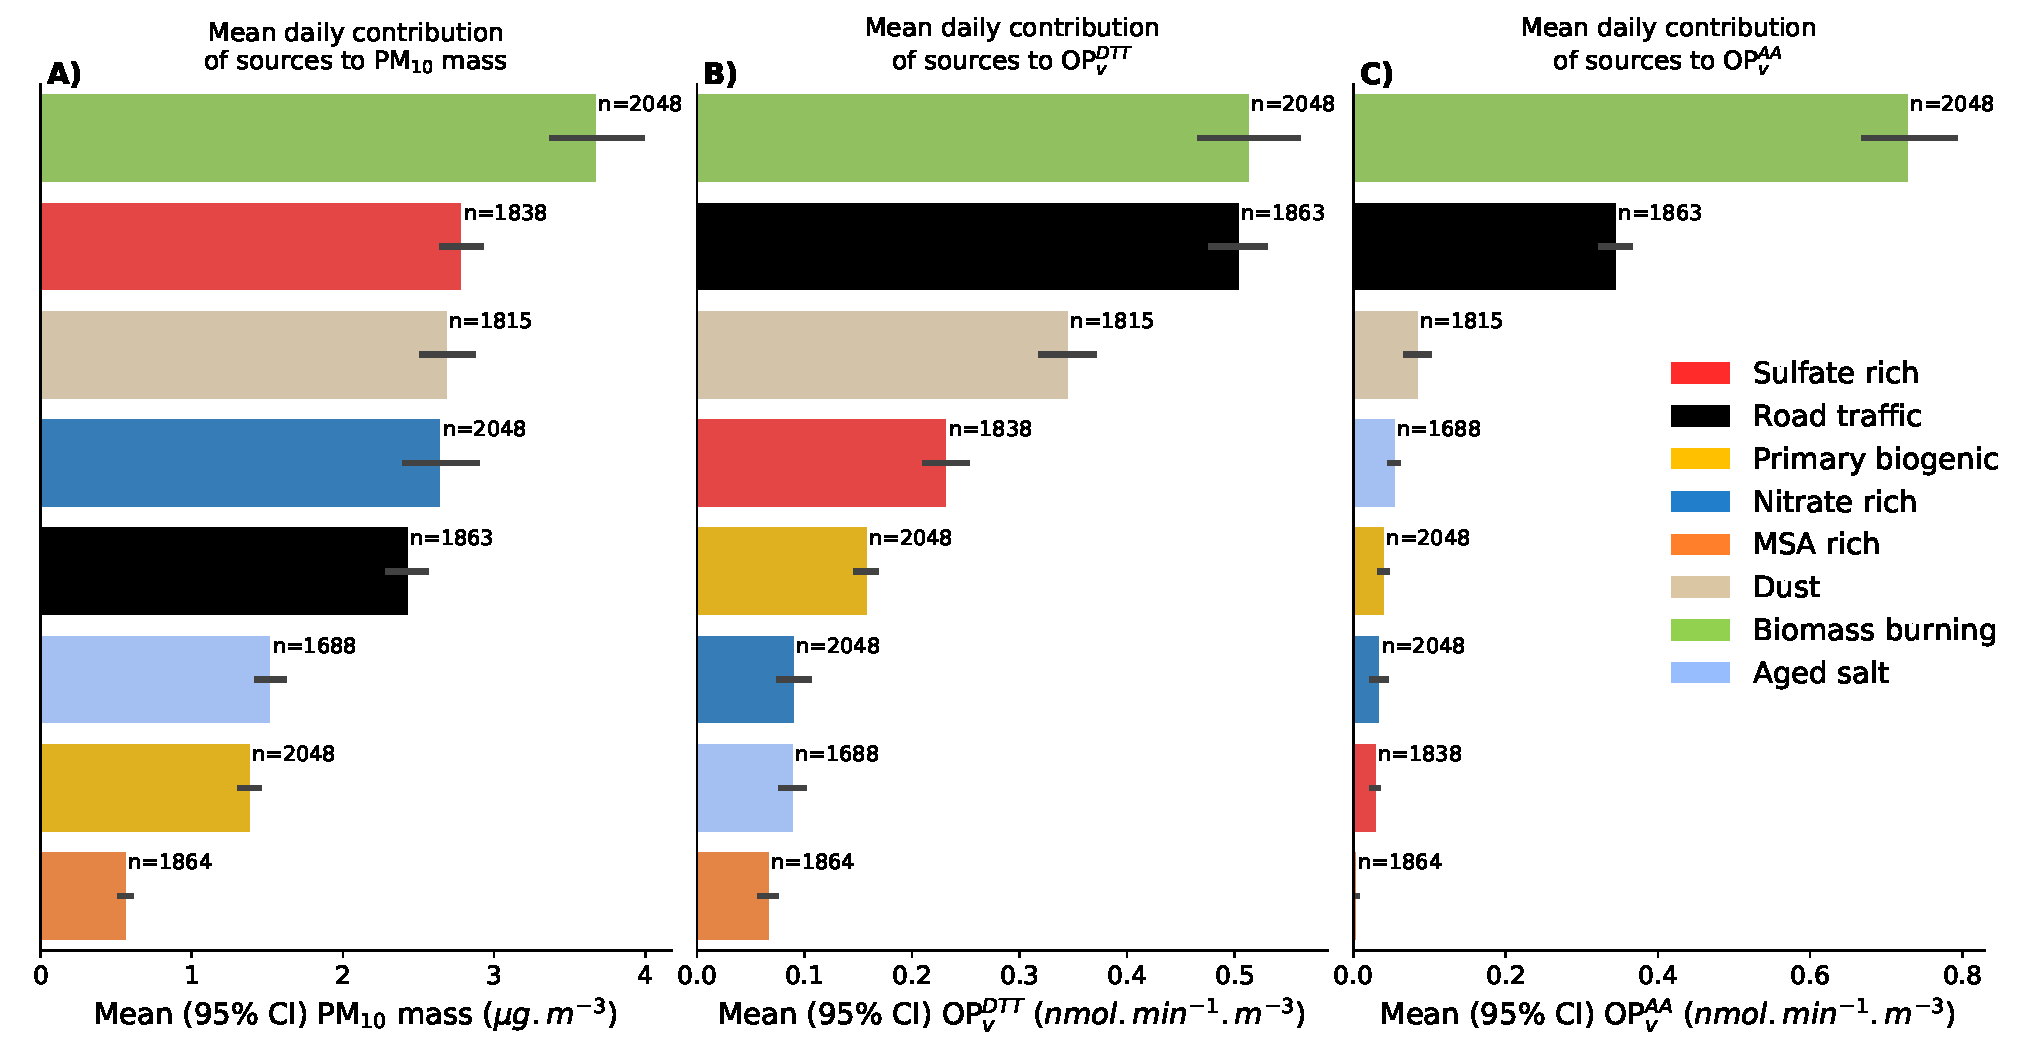
\includegraphics[width=1\linewidth]{chapter03/fig7.pdf}
    \caption{
        Estimation of the over-time uncertainties of OC* (in \si{\concum}) in the
        sulfate-rich factor at CHAM site using the BS and DISP runs. The grey line denotes
        the reference constrained run contribution, the~shaded blue area indicates the
        uncertainties (standard deviation) given by the BS and the orange shaded area the
        uncertainties given by the DISP (min max).
    }
    \label{fig:fig7}
\end{figure}

\subsection{Variability of the Chemical Profiles at the Regional~Scale}%
\label{sub:variability_of_the_chemical_profiles_at_the_regional_scale}

\subsubsection{Overall~Comparison}%
\label{ssub:overall_comparison}

In the previous sections, we discuss  the internal variability of the different factors.
Next,~similarities of all the chemical profiles identified in this study were investigated
thanks to the tools developed in the frame of the FAIRMODE (Forum for Air Quality
Modeling) activities and presented by~\textcite{belisNew2015}, based on the constrained
runs. PMF factor profiles attributed to a source category are compared among each other's
using both the PD (Pearson distance) and SID (standardized identity distance) similarity
indicators. Fewer factors identified at some sites were not considered in this assessment
analysis as they showed some mixing with other emission~sources.

Figure~\ref{fig:fig8} gives mean and standard deviation of the distances between all pair
of factor/source profiles tagged as belonging to the same category in the SID-PD space. It
results in the comparison of $n\times\frac{n+1}{2}-n$ pairs of profiles for each category,
where n is the number of profiles belonging to the same source category (see
Figure~\ref{fig:fig8}).

\begin{figure}[ht]
    \centering
    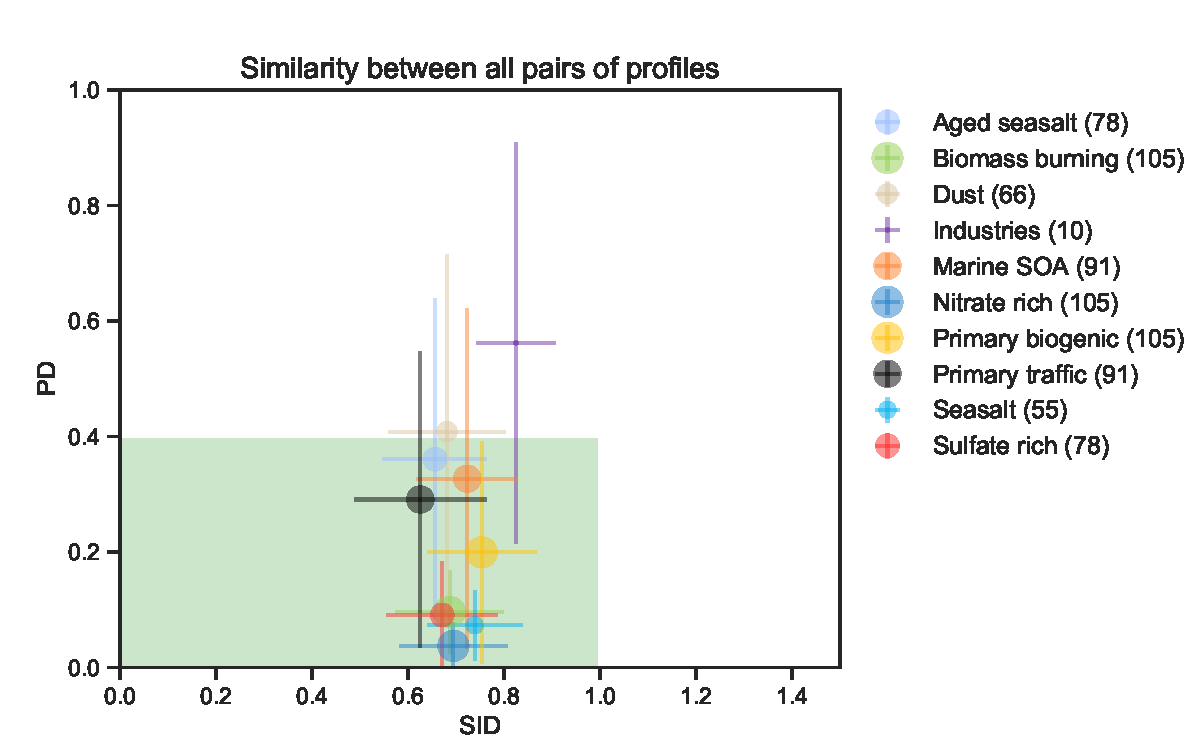
\includegraphics[width=0.8\linewidth]{chapter03/fig8.pdf}
    \caption{
       Similarity plot for all pairs of profiles belonging to the same
        factor/source category in this study. The~mean $\pm$ standard deviation
        for a given source category are plotted. The~size of the dot is
        proportional to the number of available pair of profile (from 10 to 105,
        shown in parenthesis in the legend). The~green box highlights the
        acceptable area for profile similarity according
        to~\textcite{pernigottiDeltaSA2018}.
    }
    \label{fig:fig8}
\end{figure}

First, we can see that many factor/source profiles present low PD and SID with values
(mean $\pm$ standard deviation) inside the acceptance box ($PD<0.2$ and $SID<0.8$),
indicating that they are stable over the different sites of the study.  It includes the
biomass burning, sulfate-rich, nitrate-rich, and~fresh sea-salt factors. The~primary
biogenic source also appears relatively stable at all sites but presents some
dissimilarity according to the PD metric. It suggests that this source is not yet fully
understood and need further investigation, as~recently discussed
by~\textcite{samakePolyols2019}.

Other factors seem to have more heterogeneous profiles, with~part of their values (mean
$\pm$ standard deviation) outside of the acceptance box. For~instance, differences  were
clearly observed in the few industrial chemical profiles. This is expected as such
emissions may be very local and highly variable, despite their common contents of high
concentrations of metals and metalloids. Marine SOA profiles also display site-to-site
variations and a wide range in the PD-SID space, notably for the PD metric. This factor,
mainly identified thanks to its MSA marker, may actually regroup a large diversity of
chemical species. The~low variance in the SID but high variance in the PD tends to
indicate a large discrepancy for the chemical species that represent the main mass of the
profile. A~deeper analysis (not presented here) showed  that the high variance is driven
by an observation at only three sites: GRE, CHAM and ROU. The~valley sites of GRE and CHAM
both present a larger part of OC* in their profile while, conversely, ROU presents the
lowest amount of OC* among all the sites.  Finally, the~primary traffic profile presents
the lowest SID values, but~a relatively high PD, still in the acceptable area. As~this
factor is commonly observed in RM studies and contributes substantially to the \PM{} mass,
it is discussed in detail in the following~section.

\subsubsection{A Non-Homogeneous Source: Primary~Traffic}%
\label{ssub:a_non_homogeneous_source_primary_traffic}

The primary traffic source present large variability in the SID-PD space, suggesting a
wide variety of road transport chemical profiles over France. As~a matter of fact, this
factor presents the lowest SID value of all profile while larger variabilities  were found
in the PD metric. This could be seen in the OC/EC ratio, both species being the most
abundant ones within the primary traffic factor
(Figures~\ref{fig:fig9}~and~\ref{fig:fig10}). Even  when excluding the rural site of REV,
we observed a large variability in this ratio, spanning from 0.09 to 3.31
(Figure~\ref{fig:fig10}). As~the PD is mainly sensitive to the main chemical species in
term of mass, these two compounds may explain the wide span of the PD value for this
source.  It should also be noted that the high variability in the PD may be driven by the
values for the RBX site. Indeed, despite RBX has all   22 metals in the ranges of the
other sites, the~value of OC* is extremely low compared  to others sites. The~lower
dispersion in the SID-axis highlights the relative homogeneity of the other components of
this factor. Indeed, as~shown in Figure~\ref{fig:fig9}, the~amount of metals, notably the
Fe, Cu, Al, Zn and Sb, as~well as  sulfate are relatively homogeneous over the 14 sites.
We also see that organic compounds such as levoglucosan, mannosan, MSA and polyols as well
as \ce{Na+} are almost never present in this factor, or~in a very small~amount.

The extremely high OC-to-EC ratio for REV (Figure~\ref{fig:fig10}) and the relatively
higher uncertainties estimated from the BS runs (OC*\textsubscript{BS},
\SIrange{0.000}{0.937}{\concum}; EC\textsubscript{BS}, and
\SIrange{0.0162}{0.0703}{\concum}, still close to the detection limit) indicate  low
confidence in the PMF solution for this factor at this~site.

Finally, the~primary traffic factor is the closest to the dust factor when comparing the
dust factor to all other profiles (see   Figure S1). Such results may indicate that some
resuspended dust coming from road abrasion or resuspension might contribute importantly to
the dust factors at some sites.  This may also explain the relatively low amount of trace
element in the primary traffic factor obtained at STRAS. Indeed, at~this site, we
identified a mixed factor of ``resuspended dust'',  which  may be a mixing between mineral
dust and road dust. This particular factor is not included in the ``dust'' one presented
in Figure~\ref{fig:fig8} due to it~singularity.

\begin{figure}[h]
    \centering
    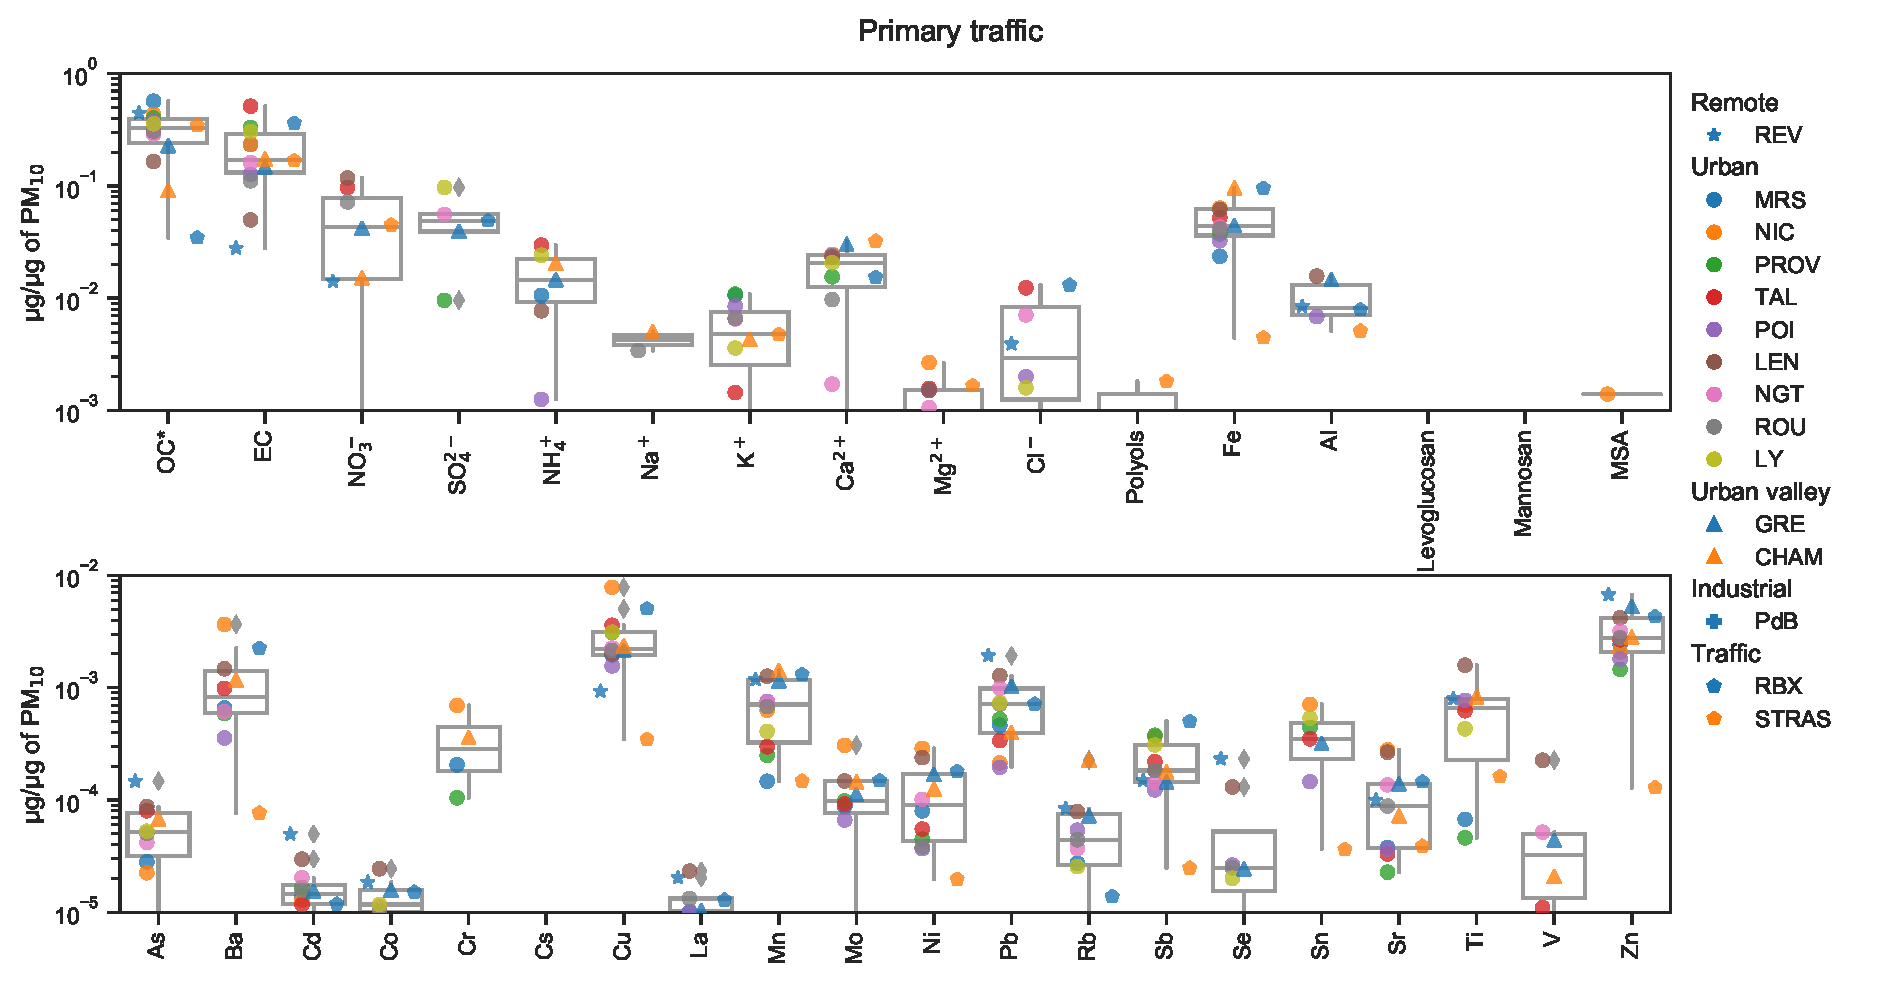
\includegraphics[width=1\linewidth]{chapter03/fig9.pdf}
    \caption{
        Chemical profiles obtained for the primary traffic factor in
        \si{\micro\gram} per \si{\micro\gram} of \PM{}. Markers refer to
        individual site and box plots show the dispersion for all sites.
    }
    \label{fig:fig9}
\end{figure}


\begin{figure}[h]
    \centering
    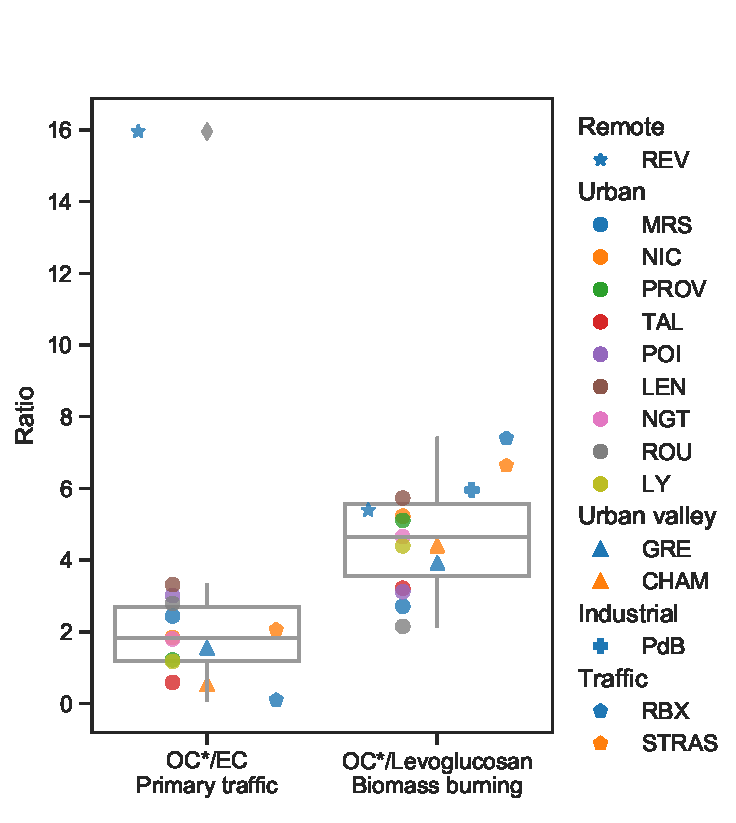
\includegraphics[width=0.5\linewidth]{chapter03/fig10.pdf}
    \caption{
        Variability of the OC-to-EC ratios and OC-to-Levoglucosan ratios obtained
        for the primary traffic and biomass burning factors, respectively.
        Markers refer to individual site and box plots show the dispersion for
        all sites.
    }
    \label{fig:fig10}
\end{figure}

\subsubsection{A Homogeneous Source: The Biomass Burning~Source}%
\label{ssub:a_homogeneous_source_the_biomass_burning_source}

Among the stable profiles, the~biomass burning is the most important source in terms of
mass contribution. As~already well reported in the
literature~\autocite{schauerMeasurement2001, schmidlChemical2008, belisCritical2013},  ~OC
is the PM dominant fraction in this source, with~a quite constant amount
(\SI{38\pm5}{\percent} of the PM mass, see Figure~\ref{fig:fig11}). Moreover, as~presented
in Figure~\ref{fig:fig6} and detailed in Figure S2, the~OC* uncertainties in this factor
is low. Concerning the tracer of biomass burning,   levoglucosan and mannosan  are present
at \SI{96\pm3}{\percent} and \SI{95\pm4}{\percent} in this profile, respectively
(Figure~\ref{fig:fig11}). Mass-wise, the~levoglucosan represents \SI{8\pm2}{\percent} of
the total PM mass. The~EC presents a wider dispersion, with~a mass concentration of
\SI{9\pm4}{\percent}. We also note a fair amount of \ce{Cl-}, as~well as \ce{K+} in this
factor, which explains \SI{14\pm19}{\percent} and \SI{32\pm13}{\percent} of their
respective total mass. Despite its contribution to the mass of biomass burning PM mass
(\SI{6\pm4}{\percent}), the~\ce{NO3^-} is clearly not mainly allocated to this source as
the biomass burning represents only \SI{7\pm5}{\percent} of the total \ce{NO3^-} mass.
Metal elements are barely present in this factor and some high discrepancy  was observed
for the different sites, with~a dispersion up to two orders of magnitude for Pb, Zn and
Mn.  It may be noted that the OC-to-Levoglucosan ratio fluctuates between 2.1 and 7.4,
with~a mean and standard deviation values of \num{4.6\pm1.5} (Figure~\ref{fig:fig10}).
Such ratios are in the 1.9--12.6 range of values previously reported for \PM{} wood
combustion samples~\autocite{schauerMeasurement2001, schmidlChemical2008}. They may
reflect the use of the different type of wood for heating purposes, as~detailed in the
same previous studies. However, we did not observe any systematic difference according to
the geographical location and/or the site typology for this source.  Overall, these
findings suggest a relatively similar wood burning emission in term of PM constituents all
over the~territory.

\begin{figure}[ht]
    \centering
    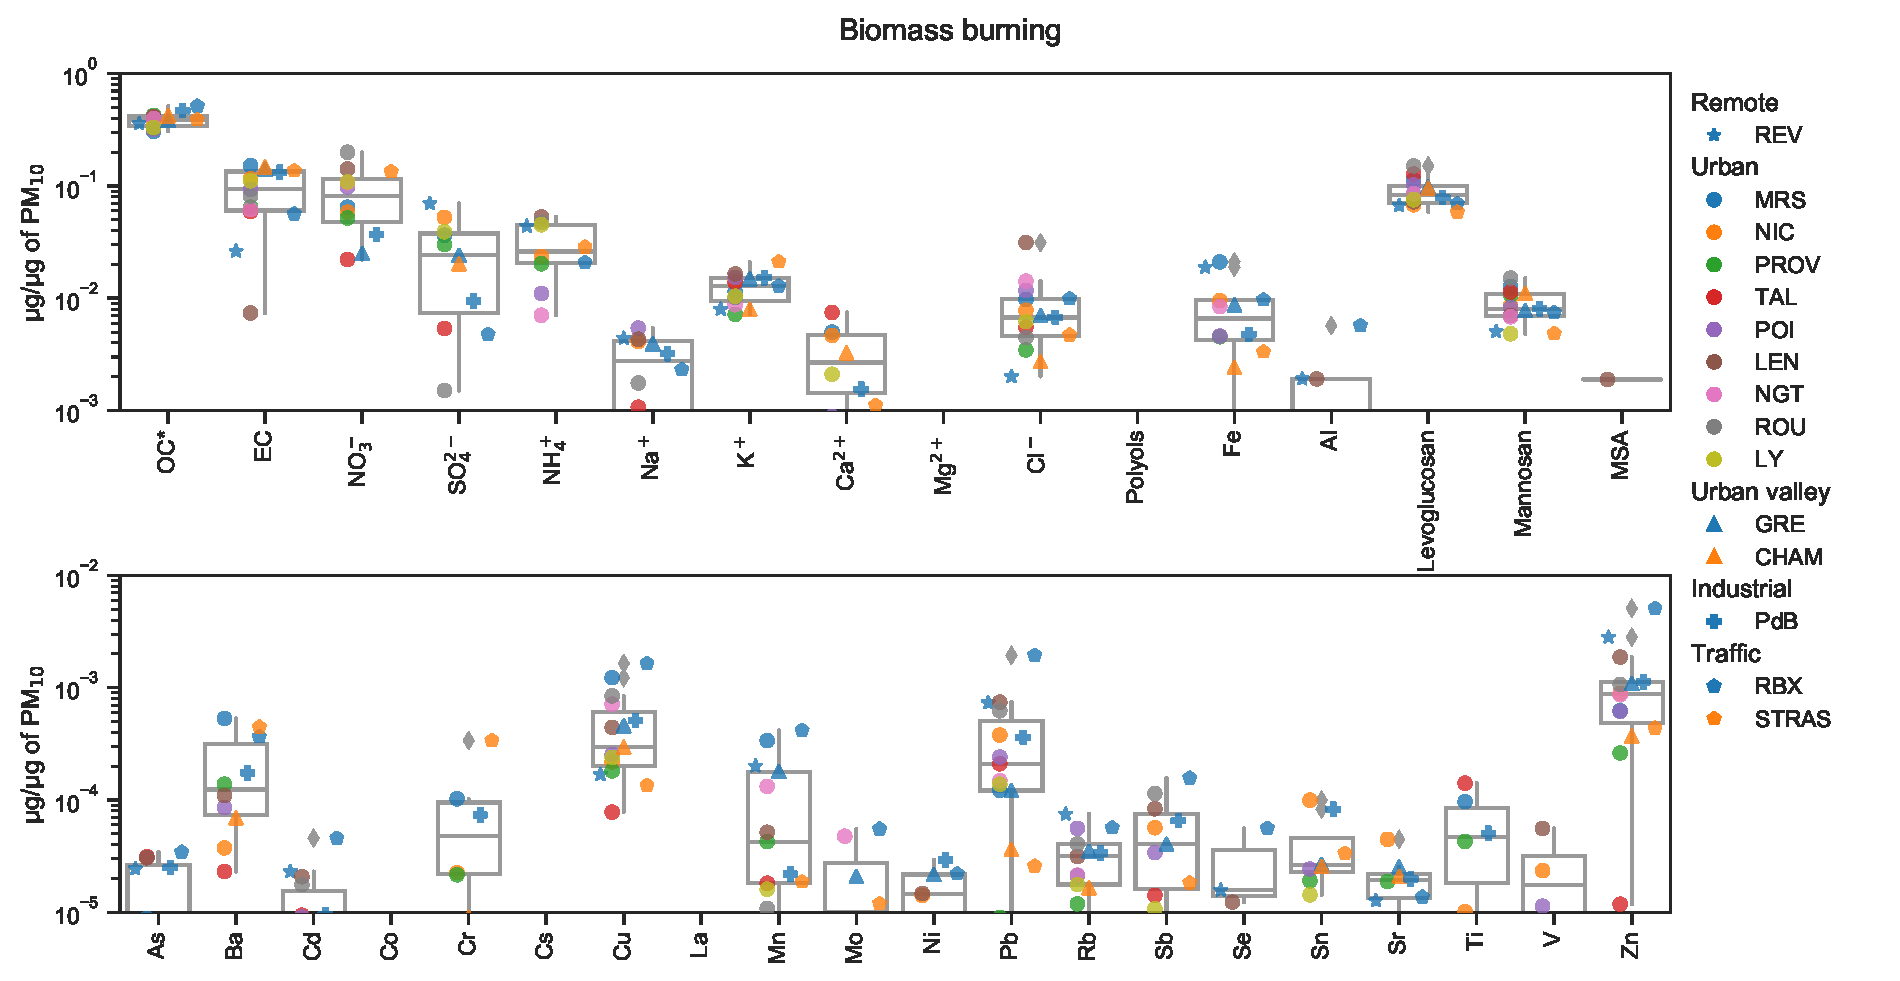
\includegraphics[width=1\linewidth]{chapter03/fig11.pdf}
    \caption{
        Chemical profiles obtained for the biomass burning factor in
        \si{\micro\gram} per \si{\micro\gram} of \PM. Markers refer to
        individual site and box plots show the dispersion for all sites.
    }
    \label{fig:fig11}
\end{figure}
%\clearpage
\section{Conclusions}%
\label{sec:conclusion}

This paper presents results obtained from PMF analyses conducted in a harmonized way and
taking advantage of datasets corresponding to more than \num{2200} samples collected at 15
different sampling sites in France. To~the best of our knowledge, this is the first study
using such a large database over several years of monitoring. Thirty-seven input variables
were selected to cover a wide range of major expected \PM{} factors and to optimize total
mass reconstruction at all sites.  The operator-related subjectivity was reduced by using
homogeneous statistical and geochemical criteria for the source discrimination
and~identification. 

Overall, the main \PM{} factors were found to be primary traffic (\SI{15\pm7}{\percent} of
the \PM{} mass on a yearly average) and biomass burning (\SI{17\pm9}{\percent}) as well as
two secondary aerosol fractions dominated by ammonium nitrate (\SI{17\pm8}{\percent}) and
ammonium sulfate (\SI{15\pm4}{\percent}), respectively. These findings are in good
agreement with what has   commonly been observed by many previous studies over Europe and
illustrates ---if still needed---the major impact of anthropogenic emissions on urban air
quality. Nevertheless, substantial contributions of mineral dusts (\SI{13\pm4}{\percent}),
fresh (\SI{6\pm2}{\percent}) and/or aged sea-salts (\SI{8\pm4}{\percent}), as~well as of
primary biogenic aerosols (\SI{7\pm3}{\percent}) are also observed at almost all sites,
reflecting that natural emissions should not be neglected as other important contributors
to \PM{} levels on a yearly~basis.

During wintertime, high contribution of the biomass burning  was observed, together with
the nitrate-rich factor in early spring (March). The~sea-salt also presents higher
contribution during this period of the year, potentially linked to stronger westerlies
winds.  In summer, all sites present important contributions from biogenic sources: the
primary biogenic and marine SOA factors.  Conversely, the~primary traffic, dust, aged
sea-salt and sulfate rich factors do not present clear seasonality~pattern.  Uncertainties
of each PMF results were investigated thanks to the bootstrap and displacement methods,
both for the base and the constrained runs. The~use of a set of constraints---taken as
limited as possible---allows to decrease these uncertainties and to strengthen the output
statistical representativity of factors commonly observed all over the French continental
territory.  The internal variability (i.e., for a given site) assessment shows high
confidence for the concentration of the main proxies of sources (i.e., specific tracers)
and for the \PM{} mass apportionment, but~larger uncertainties were  found for
concentrations of non-tracer species and caution should be taken concerning the
contributions of such chemical species to the different~factors.

Finally, the~external variability (i.e., from one site to another) was investigated thanks
to both the SID and PD metrics.  In~particular, the~discrepancy between the chemical
profiles of sources could be quantified thanks to both the SID and PD metrics, notably
showing that fresh sea salt, nitrate-rich, sulfate-rich and biomass burning factor
profiles can be considered as chemically similar at all the sites studied. Conversely,
some significant variabilities were observed for other factor chemical profiles, such as
the ones related to traffic and industrial emissions as well as mineral dusts and marine
SOA. The~latter finding is calling for the use of additional variables, such as organic
molecular markers, within~studies aiming at scrutinizing specific local sources at
individual sites and/or for a better knowledge on the origins of SOA~fractions.

Overall, results obtained in this comprehensive study may help to increase the
completeness of the SPECIEUROPE database, and~can be used to assess the contributions of
the different sources to the oxidative potential of \PM{} following methodology proposed
by~\textcite{weberApportionment2018}.



%% Acknoledgment
% This work has been conducted as part of the SOURCES project funded by ADEME
% (grant agreement no. 1462C0044). The PhD of Samuël Weber is founded by ENS
% Paris. Samples were notably collected and analyzed in the frame of various
% programs funded by the French Ministry of Environment through the CARA program
% leaded by the National Reference Laboratory for Air Quality Monitoring (LCSQA)
% and/or through programs (such as Primequal) managed by ADEME, as well as in the
% frame of actions funded by ANDRA and/or regional air quality monitoring networks
% (AASQAs). Analytical aspects were supported at IGE by the Air-O-Sol platform
% within Labex OSUG@2020 (ANR10 LABX56) and at IMT LD by the Labex CaPPA
% (ANR-11-LABX-0005-01) and CPER CLIMIBIO projects. Authors also acknowledge the
% work of many technicians and engineers in the lab. at IGE (A. Wack, C. Charlet,
% F. Donaz, F. Masson, S. Ngo, V. Lucaire, A. Vella), at Ineris (R. Aujay, A.
% Papin, V. Minguet, N. Chatellier), at IMT LD (B. Malet), and at LSCE (N.
% Bonnaire). Finally, the authors would like to kindly thank the dedicated efforts
% of many other people, notably in the AASQAs, for collecting the samples.


% %%%%%%%%%%%%%%%%%%%%%%%%%%%%%%%%%%%%%%%%%%
% \supplementary{The following are available online at \linksupplementary{s1},
% Figure S1: Similarity plot for all pair of profiles containing a  ``dust'' factor,
% Figure S2: Uncertainties of OC* in the Biomass burning profile according to BS for each site.
% In addition, \url{http://pmsources.u-ga.fr} presents interactively the whole dataset of
% this study.
% }
%
% %%%%%%%%%%%%%%%%%%%%%%%%%%%%%%%%%%%%%%%%%%
% \authorcontributions{
%     Conceptualization, J.-L.J. and O.F.; Data curation,
%     S.W. and D.S.; Formal analysis, S.W. and Dalia
%     Salameh; Funding acquisition, J.-L.J. and O.F.;
%     Investigation, A.A., L.A. and J.-L.C.;
%     Methodology, D.S.; Project administration, J.-L.J. and
%     O.F.; Resources, A.W., J.-L.B., V.J.,
%     G.G., B.M., B.R., A.H., M.D.-S. and E.C.; Software, S.W.; Supervision,
%     J.-L.J. and O.F.; Visualization, S.W.; Writing---original draft, S.W.; and Writing---review and editing, D.S.,
%     A.A., L.A., J.-L.J. and O.F.
% }


%
% %%%%%%%%%%%%%%%%%%%%%%%%%%%%%%%%%%%%%%%%%%
% \funding{
%     This work  was conducted as part of the SOURCES project funded by ADEME
%     (grant agreement No. 1462C0044). The~PhD of Samuël Weber is funded by ENS
%     Paris. Samples were notably collected and analyzed in the frame of various
%     programs funded by the French Ministry of Environment through the CARA
%     program leaded by the National Reference Laboratory for Air Quality
%     Monitoring (LCSQA) and/or through programs (such as Primequal) managed by
%     ADEME, as~well as in the frame of actions funded by ANDRA and/or regional
%     air quality monitoring networks (AASQAs). Analytical aspects were supported
%     at IGE by the Air-O-Sol platform within Labex OSUG@2020 (ANR10 LABX56) and
%     at IMT LD by the Labex CaPPA (ANR-11-LABX-0005-01) and CPER CLIMIBIO
%     projects. 
% }

% %%%%%%%%%%%%%%%%%%%%%%%%%%%%%%%%%%%%%%%%%%
% \acknowledgments{
%     The authors also acknowledge the work of many technicians and
%     engineers in the lab  at IGE (A. Wack, C. Charlet, F. Donaz, F. Masson,
%     S. Ngo, V. Lucaire, A. Vella), at~Ineris (R. Aujay, A. Papin, V. Minguet,
%     N. Chatellier), at~IMT LD (B. Malet), and~at LSCE (N. Bonnaire). Finally, the~authors would like to kindly thank the dedicated efforts of many other
%     people, notably in the AASQAs, for~collecting the~samples.
% }

%
% %%%%%%%%%%%%%%%%%%%%%%%%%%%%%%%%%%%%%%%%%%
% \conflictsofinterest{The authors declare no conflict of~interest.} 
%


\end{otherlanguage}

\printbibliography[segment=\therefsegment,heading=subbibliography]
